\documentclass[11pt, letterpaper]{amsart}
\usepackage[
            bindingoffset=0.2in,
            left=1in,
            right=1in,
            top=1in,
            bottom=1in,
            footskip=0.25in]{geometry}           
\usepackage{graphicx}
\usepackage{amssymb}
\usepackage{epstopdf}
\usepackage{subcaption}
\usepackage{placeins}
\usepackage{wrapfig}

\usepackage[backend=bibtex]{biblatex}
\addbibresource{writeup.bib}

\usepackage{hyperref}

% Force figures to stay with text
\let\Oldsection\section
\renewcommand{\section}{\FloatBarrier\Oldsection}
\let\Oldsubsection\subsection
\renewcommand{\subsection}{\FloatBarrier\Oldsubsection}
\let\Oldsubsubsection\subsubsection
\renewcommand{\subsubsection}{\FloatBarrier\Oldsubsubsection}

\DeclareGraphicsRule{.tif}{png}{.png}{`convert #1 `dirname #1`/`basename #1 .tif`.png}
\graphicspath{{./notebooks/figs/}}

\title{STAT 215A, Final Project\\Classifying ciTBI in Youth}
\author{Mark Oussoren, Sahil Saxena, Hyunsuk Kim, Florica Constantine}
\email{\{mark\_oussoren, sahilsaxena18, hyskim7, florica\}@berkeley.edu}
\date{2021 December 10 Friday}  

\begin{document}
\maketitle

\section{Introduction}

% How can we best vet and/or improve the clinical decision rule for your given problem? Most importantly, the clinical decision rule should be highly predictive and minimize the amount of missed diagnoses (i.e. have a very high sensitivity). It should also be easy-to-use, using variables that clinicians can readily have access to when making their decisions. Finally, the interpretability of the rule helps to check whether its predictions will make sense for new patients and makes it easier to apply in new settings.

Clinically-important traumatic brain injuries, hereafter referred to as ciTBIs, are both commonplace and require immediate medical attention. However, diagnoses often require a CT scan to confirm the presence of a TBI \cite{brenner2002estimating}. In children, this need is problematic, as the radiation from a CT scan can lead to long-term adverse affects; hence, given a child presenting with a potential TBI, it is desirable to find a way to decide whether they actually need a CT scan. Note that forgoing a CT scan in the presence of an actual TBI is also undesirable. In this report, we revisit the data from \cite{kuppermann2009identification} and derive an updated decision rule for identifying which child patients need a CT scan. That is, given several descriptors of a patient's status, we translate these into numerical features that we may feed into a statistical model to predict the need for a CT scan. 

In this report, we begin by discussing the data in section \ref{sec:data}. We discuss its collection in section \ref{ssec:datacollect} and some of its details in section \ref{ssec:datamean}. We perform a lengthy exploratory data analysis (EDA) in section \ref{ssec:datamean}. In section \ref{sec:model}, we fit models to the data and interpret the results. We discuss the baseline model from \cite{kuppermann2009identification} in section \ref{ssec:baseline} and results in section \ref{ssec:results}. We perform an analysis with an alternative data split (explained later) in section \ref{ssec:verbal}. Finally, we present conclusions in section \ref{sec:conclusions}. 

\section{Data}\label{sec:data}

\subsection{Data collection} \label{ssec:datacollect}

% What are the most relevant data to collect to answer the question in (1)? Ideas from experimental design (a subfield of statistics) and active learning (a subfield of machine learning) are useful here. The above question is good to ask even if the data has already been collected because understanding the ideal data collection process might reveal shortcomings of the actual data collection process and shed light on analysis steps to follow. The questions below are useful to ask: How were the data collected? At what locations? Over what time period? Who collected them? What instruments were used? Have the operators and instruments changed over the period? Try to imagine yourself at the data collection site physically.

The authors in \cite{kuppermann2009identification} collected data in a prospective cohort study from 43,499 patients younger than 18 years of age that visited a hospital within 24 hours of experiencing head trauma. The study was run across 25 pediatric emergency departments over a span of approximately 2 years, where the last few months were used to collect samples for validating the decision rules derived in the original study. Only patients with GCS (Glasgow Coma Scale) scores of 14 or 15 were considered; those with scores 13 or less were enrolled but were not grouped with the others. For each patient, a trained investigator or other medical personnel recorded various prespecified details, e.g., mechanism of injury, medical history, and responses to standardized questions about the presence of several symptoms or signs of head trauma on a standardized data form. 

For a small subset of patients (approximately 4\%), a second assessment was performed for quality control purposes--note that we do not use this information, but that its presence is reassuring. Note that there will likely be uncaught entry errors or errors arising from incorrect patient reporting in the data, as well as subjective biases in reporting (e.g., what constitutes a severe injury might differ between physicians and parents). All of these are sources of randomness in the data. Moreover, there will be natural differences arising from the different hospitals and the different populations that they serve---we are not privy to this information, but it is a source of potential batch effects. Nonetheless, we believe that apart from age groupings (discussed later), all of the data may be analyzed together. Moreover, each sample in the data comes from a unique person-event combination, that is, there are no repeated samples or temporal dependencies that we know of. It is certainly possible that a patient is in the data twice, but we believe that this is likely a very rare event, if it occurs at all. 

\subsection{Meaning}\label{ssec:datamean}

% What does each variable mean in the data? What does it measure? Does it measure what it is supposed to measure? How could things go wrong? What statistical assumptions is one making by assuming things didn’t go wrong? (Knowing the data collection process helps here.) Meaning of each variable -- ask students to imagine being there at the ER and giving a Glasgow coma score, for example, and also a couple of variables -- ask students what could cause different values written down. How were the data cleaned? By whom?

In this section, we discuss some of the important variables and features in the dataset. 

The study defined death, a hospital admission of over 2 days, intubation for over 24 hours, or the need for surgery following a CT scan as a positive, ciTBI outcome. Other patients were assigned to the negative outcome; to find missed positives, the study coordinators performed telephone surveys to follow up with parents and tracked followup visits. If a positive outcome was missed, the patient's label was updated to positive. 

An important variable in this data set is the GCS score. The Glasgow Coma Scale (GCS) is a common scoring system used in emergency departments to determine a patient's level of consciousness by rating their ability to pass certain tests for eye and motor movement along with verbal ability \cite{teasdale2014glasgow}. The scores from each of these three categories are summed to form a total GCS score, valued in 3-15. The lower the score a patient has in each category leads to a lower GCS total score (meaning the worse a state a patient is in). 

Note that several variables or descriptors in the study require the ability to converse with the child for assignment, e.g., the presence of a headache or whether or not the child is suffering from amnesia. Similarly, a GCS score for a pre-verbal child is also calculated by slightly different metrics than those for an adult. Judging verbal ability, especially, is different with a condition like `inappropriate words' being instead assessed as `cries of pain' for those children who are pre-verbal. Even motor ability has some conditions assessed differently such as looking for `spontaneous movement' rather than `follow commands' in preverbal children. Hence, as in \cite{kuppermann2009identification}, we chose to separate patients under the age of two (presumed pre-verbal) from those aged two or older (presumed verbal) in their analysis. Moreover, as children under the age of two are more sensitive to radiation, it is reasonable to consider this group separately \cite{brenner2002estimating}. Note that this is not a perfect grouping as some children will be verbal by age two and some children are not verbal after age 2 (we look into this in our stability analysis) but, nonetheless, it is good developmental benchmark \cite{blackwell2007pediatric}.

The variables in our data are all categorical or ordinal, except for age (however the categorial version of the age variable where it was discretized by $< 2$ years old and $\geq 2$ years old was used in all our analyses for the reasons stated above). While it would be ideal if instead the continuous version of the variables were reported and they were not pre-sorted into sometimes arbitrarily chosen categories (i.e. the length of a seizure is binned as  $< 1$ min, $1 - 5$ min, $5 ‐ 15$ min, and $> 15$ min), we are restricted to the categorical data. 

Several binary indicator variables exist in the dataset, looking at, respectively, whether a child suffered a loss of consciousness, seizure, headache, vomiting, altered mental state, palpable skull fracture, basilar skull fracture, hematoma, trauma above the clavicles, neurological deficits, or other (non-head) substantial injuries. Each of these variables also has more specific follow up questions, e.g. the type of basilar skull fracture if it is indicated a patient has one. Other important variables included in our data set are the injury mechanism, injury severity, and whether the child is acting normally, is intubated, is paralyzed, and/or is sedated.

Lastly, we also have several meta variables such as patient number, race, ethnicity, gender, position of medical professional, and certification of medical professional. These variables do not affect whether a patient will be positive for ciTBI. However, they may be useful to look at after our analyses are complete in case they are acting as a proxy for something deeper that is taking place but should not be used as feature inputs to our models.

\subsection{Exploratory Data Analysis} \label{ssec:eda}

\subsubsection{Outcome}

First, we looked at our outcome variable and noted that there were 20 patients that had a missing value. Note, there is a discrepancy where with \cite{kuppermann2009identification}, where they mention 18 not 20 patients have a missing value. The reasoning for this difference could not be resolved. Of these 20 patients, 17 of them are negative for all four of the variables making up our outcome (death, hospital admission of longer than 2 days post CT, intubation for more than 24 hours, or neurological surgery). We thus assign these patients as being negative for a ciTBI. For the three remaining patients, they had missing values for one or more of the four outcomes and were dropped. The last remaining patient had missing values for intubation and death by TBI. We impute all three of these patients to also be negative for ciTBI after talking to our clinician collaborators, who suggest it is unlikely death by TBI or intubation would not be marked on a medical form if they did in fact take place. The proportion of each of the four outcomes is shown below in Figure \ref{fig:outcome_type}. We can see that the vast majority of people were positive for a prolonged hospital stay.
\begin{figure}
	\centering
	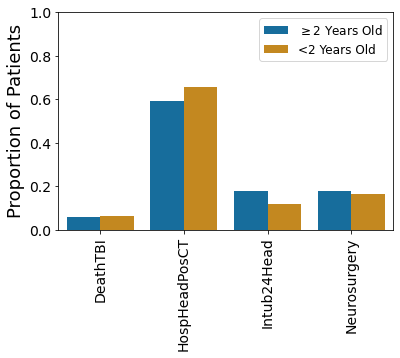
\includegraphics[width=0.5\textwidth]{outcome_type.png}
	\caption{Outcome type for ciTBI patients by age group}\label{fig:outcome_type}
\end{figure}


\subsubsection{GCS Scores}

From \cite{kuppermann2009identification}, we learned that it is not controversial to perform a CT scan for patients with a GCS score ranging from 3 to 13 as in this group the risk of finding a TBI on a CT is more than 20\%. For our data set, we looked at the proportion of patients positive for ciTBI with a GCS scores in the range of 3-13 and also for those in the range for 14-15 in Figure \ref{fig:GCSClass}. Looking at this, we can see that 40\% of patients with a GCS score in the range of 3 to 13 were positive for ciTBI versus only 0.8\% of those with a GCS score of 14 or 15---this is quite a dramatic difference. However, we wanted to know if separating the GCS score into classes with a cutoff GCS score of 14, in particular, was the best possible split. We broke up the previous plot further into individual GCS scores (Figure \ref{fig:GCSTotal}). We can see that, in general, the lower the GCS score the higher the proportion is for a patient to be positive for ciTBI---as expected. Even at a GCS of 13, 20\% of patients were positive for ciTBI. Thus, keeping the current cutoff of 3-13 and 14-15 as the two separate GCS classes seems reasonable. Hence, we remove any patients that have a GCS in the range of 3-13 (969 total patients), as the risk of having a positive ciTBI is too high and any reasonable or acceptable (to a practitioner) decision rule would suggest always performing a CT scan for this group.
\begin{figure}
	\begin{minipage}[b]{0.5\linewidth}
		\centering
		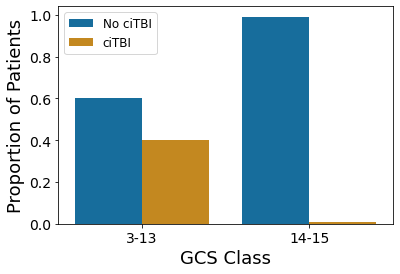
\includegraphics[width=\textwidth]{GCSClass_prop.png}
		\subcaption{Proportion of patients with ciTBI by age and GCS Class}\label{fig:GCSClass}
	\end{minipage}%
	\begin{minipage}[b]{0.5\linewidth}
		\centering
		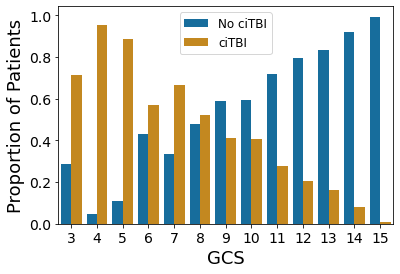
\includegraphics[width=\textwidth]{GCSTotal_prop.png}
		\subcaption{Proportion of patients with ciTBI by age and GCS Score}\label{fig:GCSTotal}
	\end{minipage}
	\caption{GCS Score and ciTBI}\label{fig:GCS}
\end{figure}


\subsubsection{Data Missingness}

Next, we look at the rate of missingness for each feature in Figure \ref{fig:cov_missing}. We note that the features `Dizzy' and `Ethnicity' are missing in more than 35\% of patients. On the data form, ethnicity asks whether the patient is hispanic or not and may potentially be skipped over by a patient if they fill in the race field instead (or if they are too young to fill out a form and the medical personnel does not want to guess). However, we are already considering ethnicity to be a meta variable and did not use it in our analyses . After speaking with the clinicians, we learned that notating whether a patient is dizzy or not is not very relevant in diagnosing TBI and it is also a very subjective variable: it is highly susceptible to change from patient to patient based on their own personal definition of feeling dizzy. Thus, as there is no objective way to compare or impute this variable, we decided to drop it.

For the other variables with missingness, they were either imputed with what a `healthy' response would be, e.g. a `No' value would be imputed for missing paralyzed or sedated values. Otherwise, the response that was the mode was used for variables where there was no clear `healthy' response. e.g. hematoma size.

Many variables have a parent question such as `Seiz' for seizure that have follow up question such as the length of the seizure. If a patient has a response of `No' for seizure then in the form `Not applicable' is often marked for each follow up question. Without loss of generality, we convert these `Not applicable' answers to be `No' to make analyses easier to perform.

We further note that the majority of patients have only around 1\% of data features missing, and at most still under 20\% (Figure \ref{fig:sample_missingness}) and thus we do not drop any patients from our analyses.
\begin{figure}
	\begin{minipage}[b]{0.5\linewidth}
		\centering
		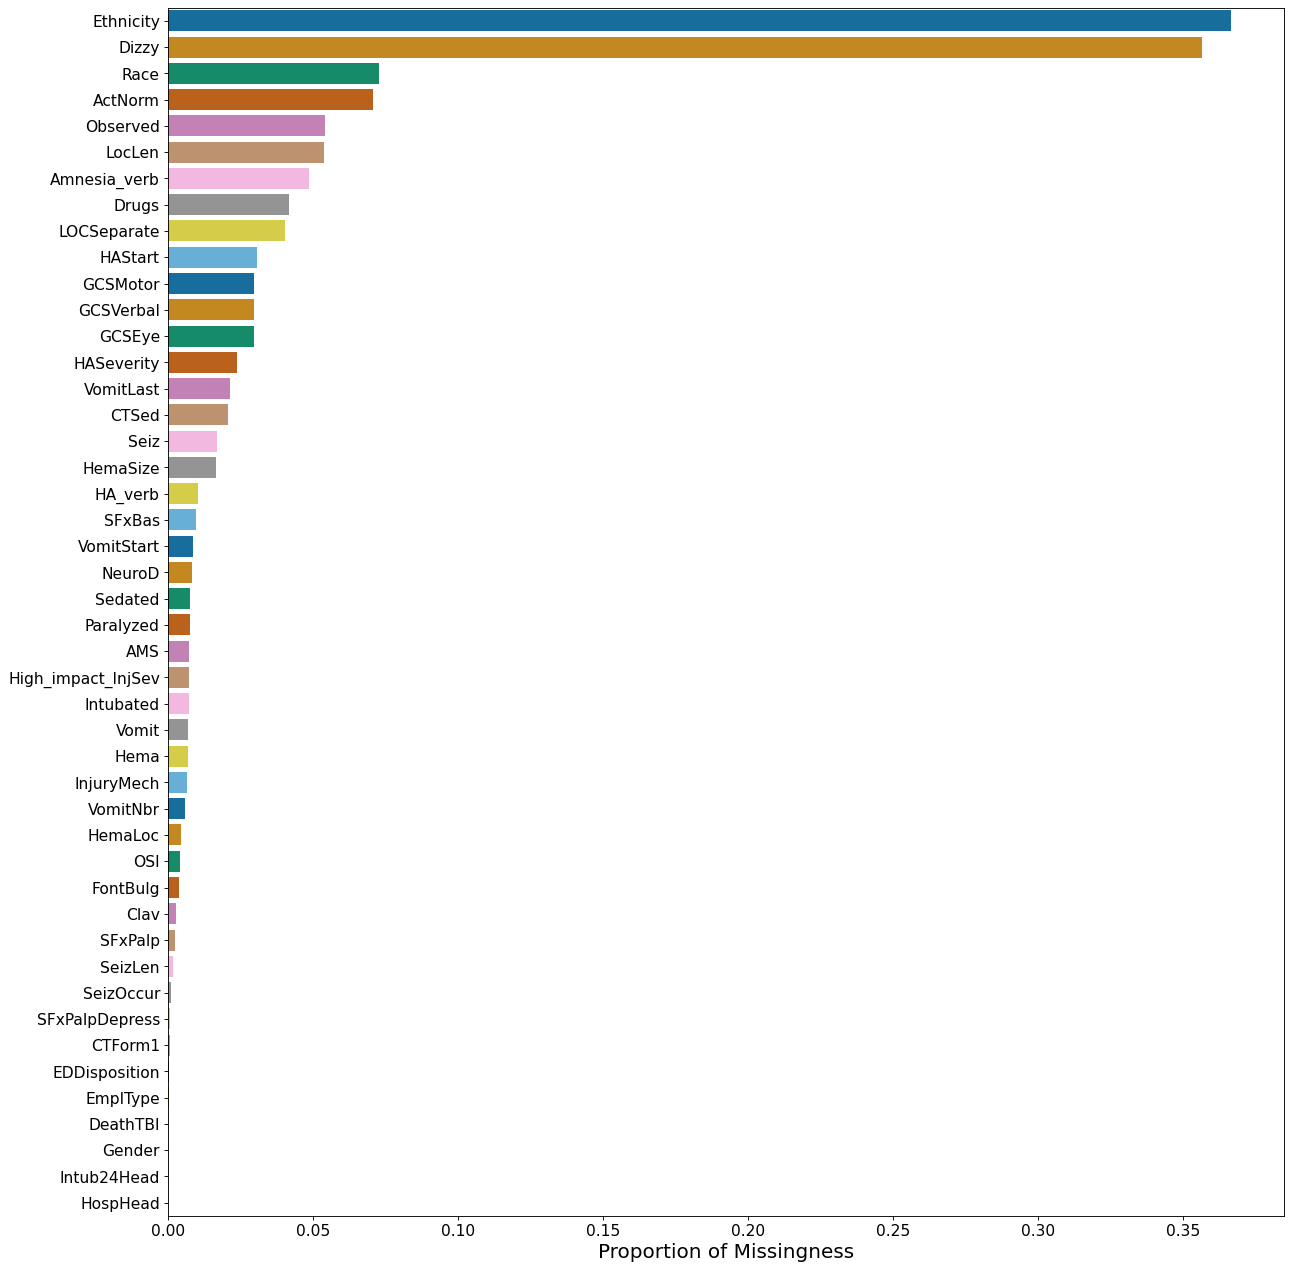
\includegraphics[width=\textwidth]{covariate_missingness.png}
		\subcaption{Fraction of samples missing a given feature}\label{fig:cov_missing}
	\end{minipage}
	\begin{minipage}[b]{0.5\linewidth}
		\centering
		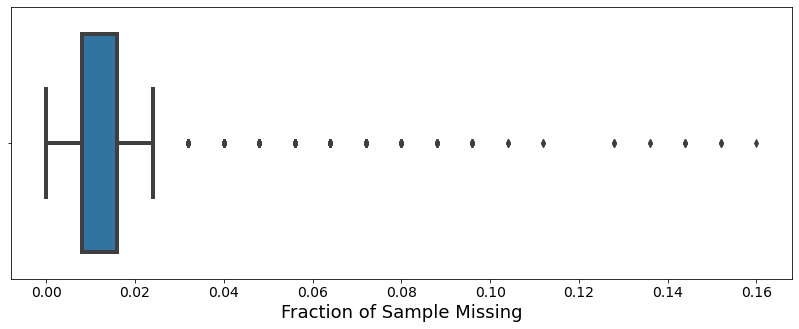
\includegraphics[width=\textwidth]{sample_missingness.png}
		\subcaption{Fraction of entries missing within a sample}\label{fig:sample_missingness}
	\end{minipage}
	\caption{Missingingness in the data}\label{fig:missing_agg}
\end{figure}

\subsubsection{Age Class Cutoff}

The age was a major factor in \cite{kuppermann2009identification} for creating a decision rule. Two rules were created based on age categories of $< 2$ and $\geq 2$ years of age. We can see a large portion of the patient population in our data set is younger and around 2 years of age in Figure \ref{fig:age_dist}.
\begin{figure}
	\centering
	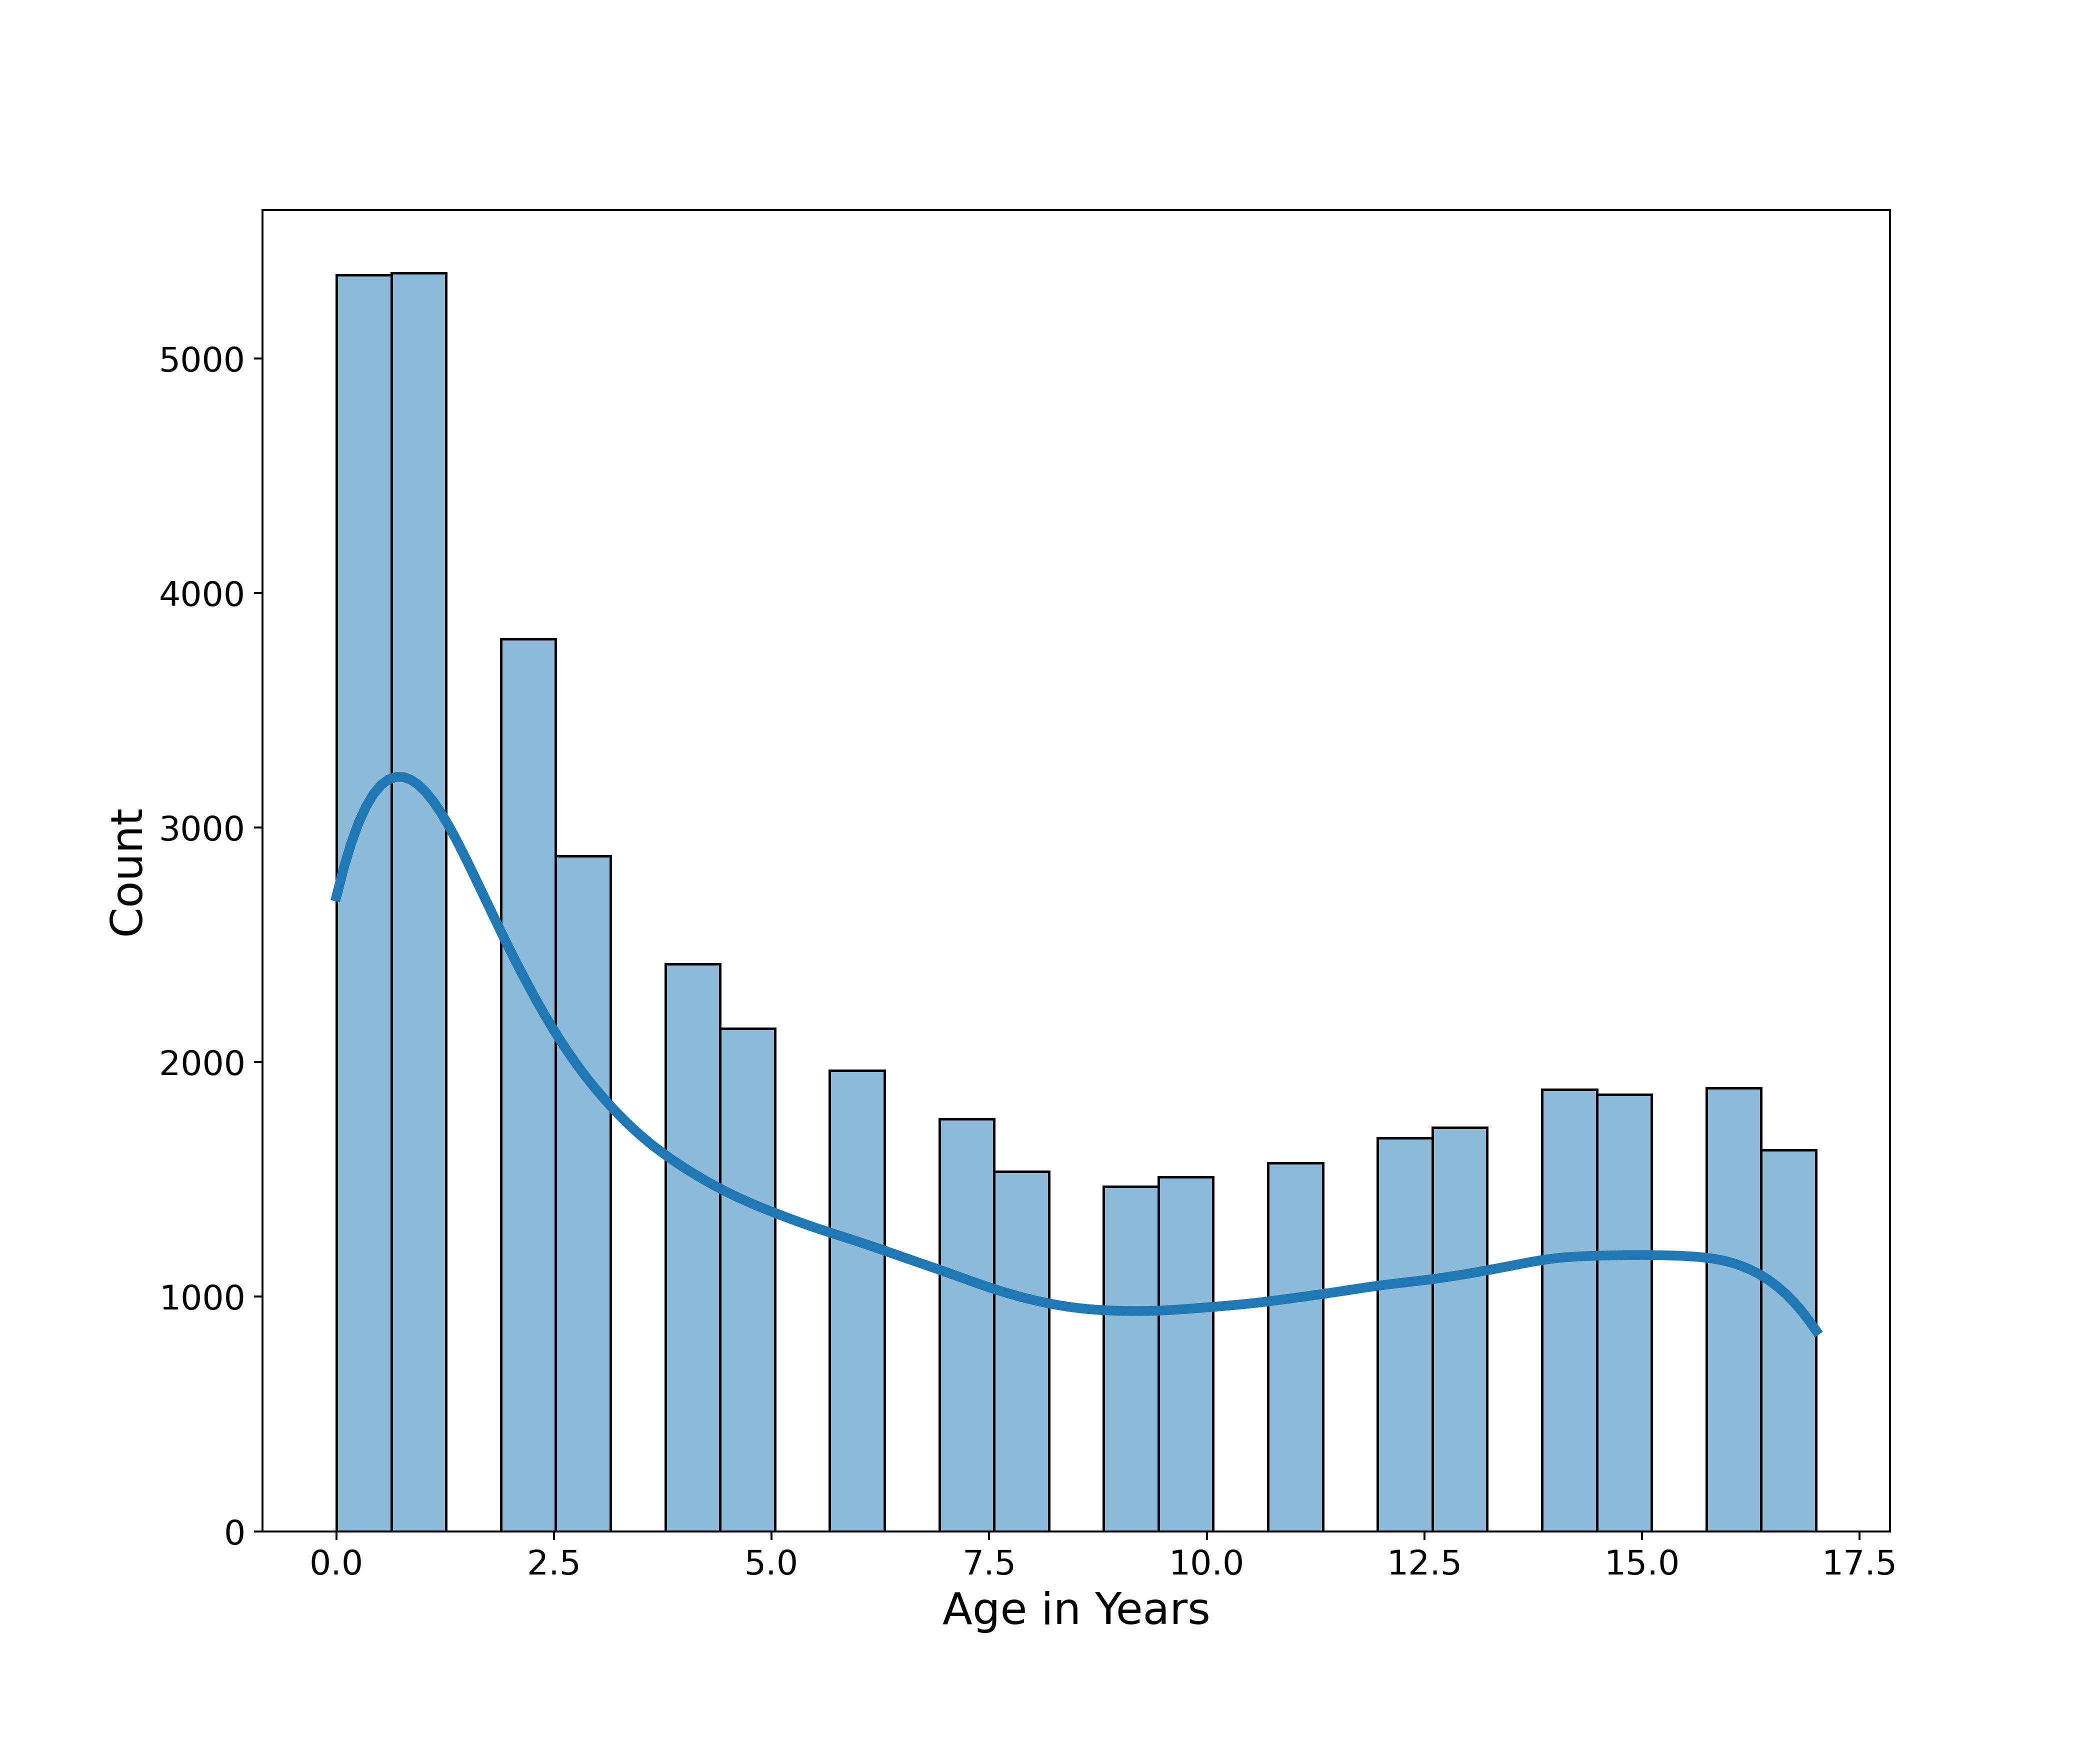
\includegraphics[width=0.5\textwidth]{age_dist.png}
	\caption{Age Distribution}\label{fig:age_dist}
\end{figure}

Besides radiation exposure risks, one reason to demarcate age at $2$ years is because of verbal ability: below this age, children typically do not talk coherently if at all. We wanted to check the number of pre-nonverbal subjects at each age to see if two years old is actually a good cutoff age for being verbal. In Figure \ref{fig:preverbal}, we can see that actually there are still a large proportion of subjects that are pre-verbal at ages 2 and 3 when calculated based on responses for whether a patient had a headache or amnesia in the data. Both of these features are the closest proxy we have to knowing how many pre-verbal patients are in our data set, as a binary variable for being pre-verbal does not exist. It is reassuring that the proportions between the two for each age are extremely similar. 
\begin{figure}
	\begin{minipage}[b]{0.5\linewidth}
		\centering
		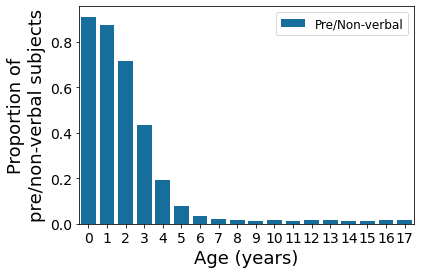
\includegraphics[width=\textwidth]{amnesia_preverbal.png}
		\subcaption{Preverbal response to Amnesia question}\label{fig:amnesia_preverbal}
	\end{minipage}%
	\begin{minipage}[b]{0.5\linewidth}
		\centering
		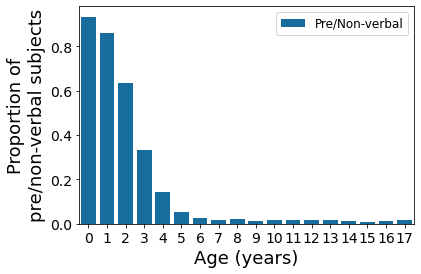
\includegraphics[width=\textwidth]{headache_preverbal.png}
		\subcaption{Preverbal response to Headache question}\label{fig:headache_preverbal}
	\end{minipage}
	\caption{Preverbal responses to Amnesia and Headache questions}\label{fig:preverbal}
\end{figure}



\subsubsection{Distribution of Features by Age}

Next, we look at the occurrence of ciTBI in each of our two age categories in Figure \ref{fig:age_by_outcome}. We can see that the proportion of ciTBI in each age category is very close to being the same. The proportions looking at injury severity in Figure \ref{fig:age_by_injury_severity} are similar across age category.
\begin{figure}
	\begin{minipage}[b]{0.5\linewidth}
		\centering
		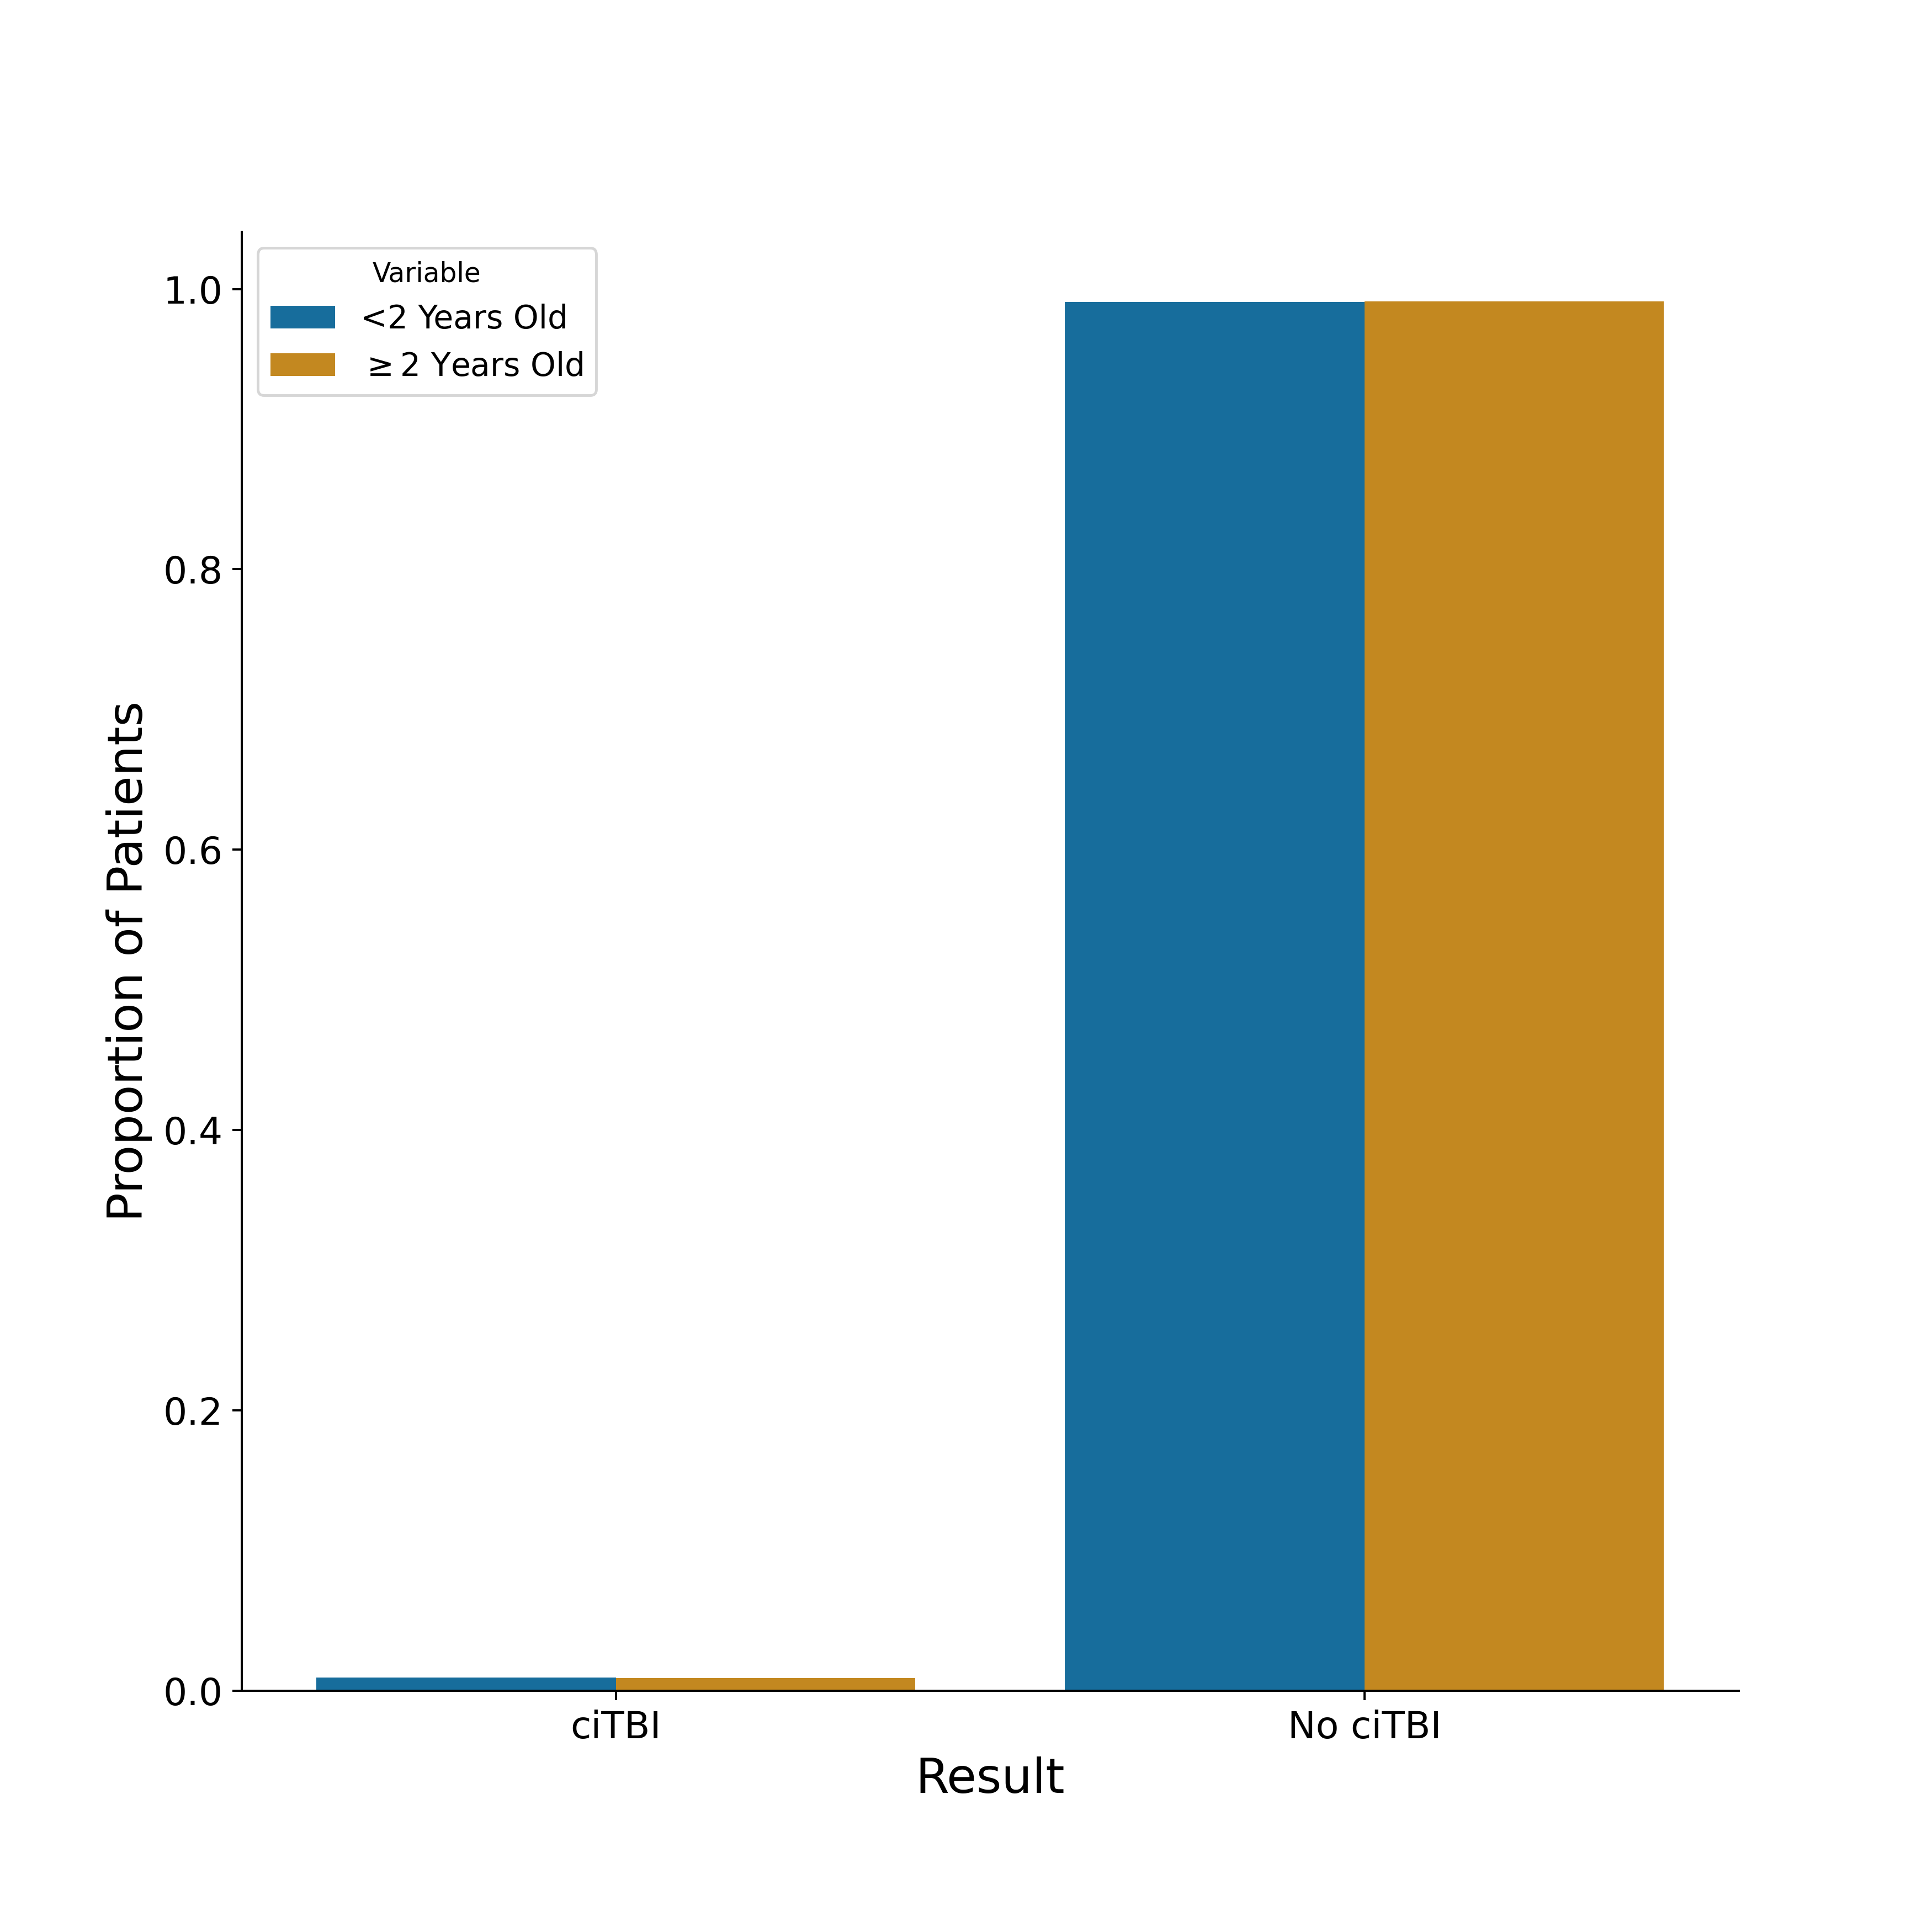
\includegraphics[width=\textwidth]{age_comparison_by_group.png}
		\subcaption{Proportion of outcomes grouped by age}\label{fig:age_by_outcome}
	\end{minipage}%
	\begin{minipage}[b]{0.5\linewidth}
		\centering
		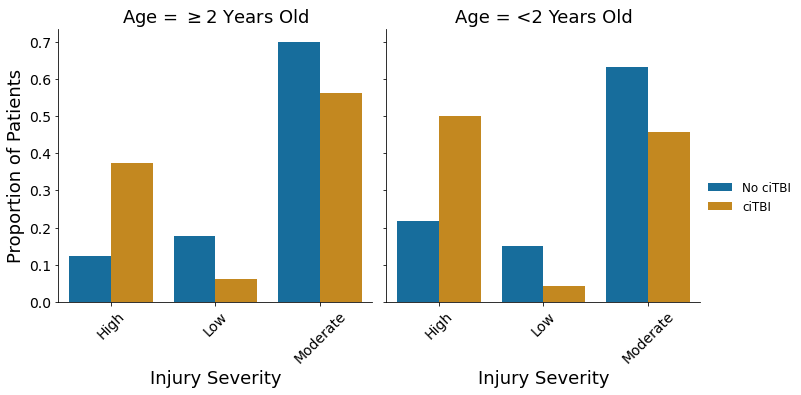
\includegraphics[width=\textwidth]{age_by_injuryseverity.png}
		\subcaption{Proportion of injury severity grouped by age}\label{fig:age_by_injury_severity}
	\end{minipage}
	\caption{Outcome and Injury Severity}\label{fig:age_distributions}
\end{figure}

However, there may still be other variables with different proportions of positive ciTBI across age categories in Figure \ref{fig:age_covariate}. That is, for each age category and for each outcome, we look at the proportion of patients with the indicated symptom. This exercise might be indicative as to whether such a variable would potentially lead to a different decision rule between the two groups. We can see that the proportion of patients with ciTBI are noticeably different between age $<2$ and age $\geq 2$ for 'Vomit' and 'OSI' (other non-head injury). Also, we note that the variables measuring amnesia and headache cannot be answered by those that are pre-verbal and thus may be useful in a decision rule for those over age 2 but not under.
\begin{figure}
	\centering
	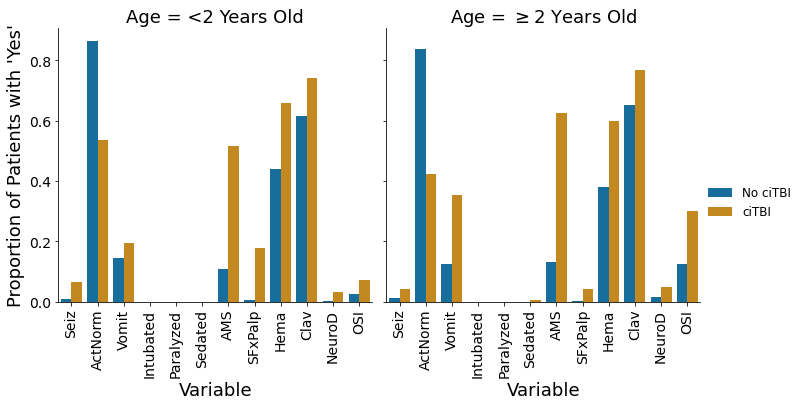
\includegraphics[width=\textwidth]{covariate_by_age.png}
	\caption{Proportion of positive feature identifiers by outcome (ciTBI) and age}\label{fig:age_covariate}
\end{figure}

\subsubsection{Correlation of Features to Outcome}

Next, we examine whether any of the features are particularly correlated to the outcome by calculating the Spearman's $\rho$ coefficient on the ordinal variables against the binary outcome. We can see in Figure \ref{fig:spearman_corr_to_outcome} that none of the features are well correlated with the outcome. A maximum correlation coefficient of 0.12 is attained by the altered mental state feature.
\begin{figure}
	\centering
	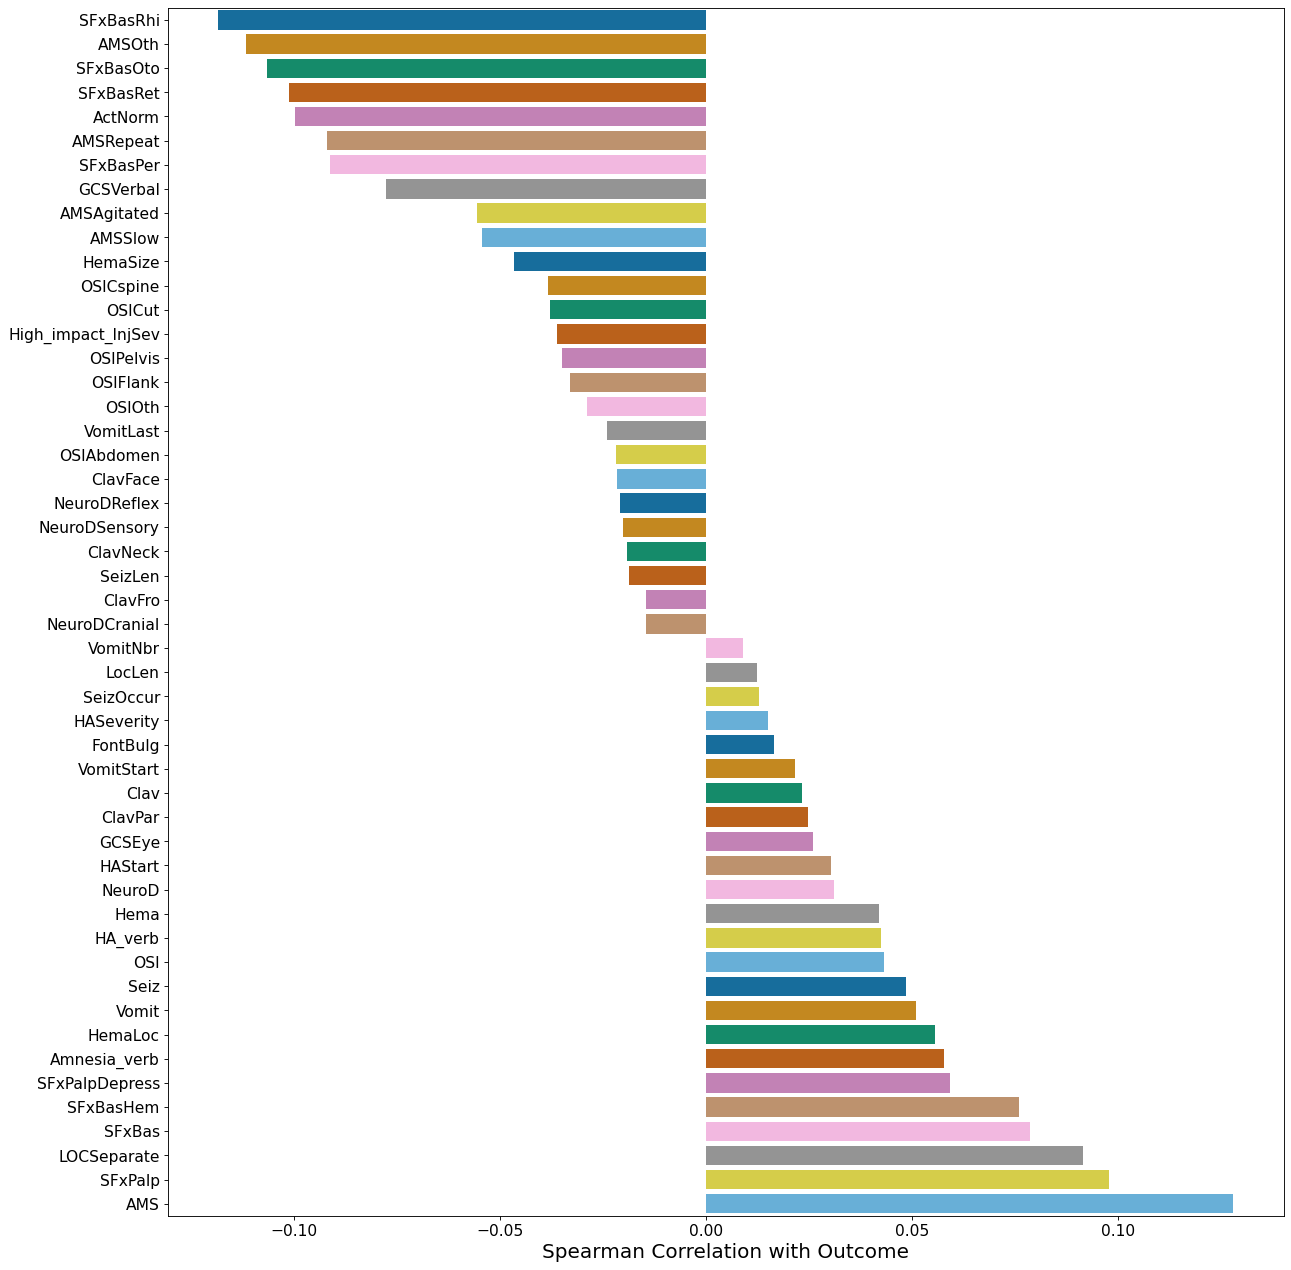
\includegraphics[width=0.5\textwidth]{spearman_corr_to_outcome.png}
	\caption{Spearman Correlation of Features to Outcome}\label{fig:spearman_corr_to_outcome}
\end{figure}

\subsubsection{Principal Component Analysis}

We perform Principal Component Analysis (PCA) on the one-hot encoded data \cite{pearson1901liii}. In Figure \ref{fig:pca_cum_var}, we see that the nearly all of the variance is explained by the first 100 components, and that the first few components capture most of the variance (the first two components explain 13\%, the first five explain 30\%, and the first twenty explain 50\% of variation in the data). That is, noting that the PCA eigenvalues (variances) decay rapidly, we might believe that this dataset behaves like a low-rank signal plus noise. 

In Figure \ref{fig:pca}, we project the one-hot encoded data to two dimensions to study if the classes (age and outcome) are visually separable. First, we see that the classes do not separate, but that there are two distinct clusters in the data---since the data were taken from 25 hospitals and that there was no laboratory or experimental processing of the data, we did not suspect a batch effect (there would only be two potential batches). Instead, we see that the presence of an OSI (other, non-head-related injury) leads to the two clusters. Note that the prevalence of OSI in the data is low (10\%), but that it is enough to strongly affect the results of PCA. We will keep this in mind when doing our analyses and look to see if the majority of the misclassified points come from patients who had an OSI injury. This means we may want to consider forming a separate decision rule for this subgroup of the patient population.
\begin{figure}
	\centering
	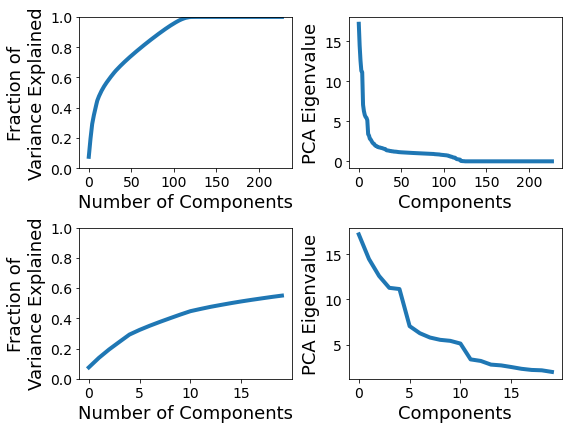
\includegraphics[width=\textwidth]{pca_cum_var.png}
	\caption{PCA: Cumulative Variance Explained and PCA Eigenvalues}\label{fig:pca_cum_var}
\end{figure}
\begin{figure}
	\begin{minipage}[b]{0.5\linewidth}
		\centering
		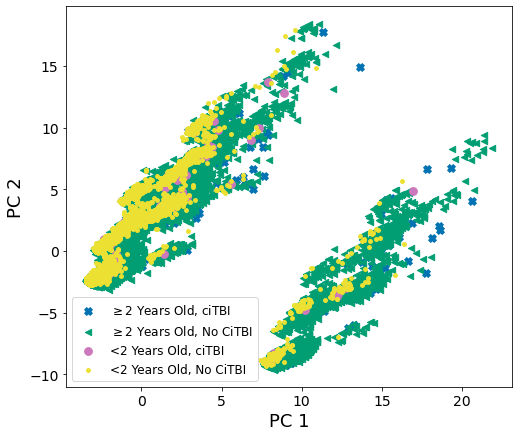
\includegraphics[width=\textwidth]{pca_age_outcome.png}
		\subcaption{2-dimensional PCA projection colored by Age and Outcome}\label{fig:pca_age_outcome}
	\end{minipage}%
	\begin{minipage}[b]{0.5\linewidth}
		\centering
		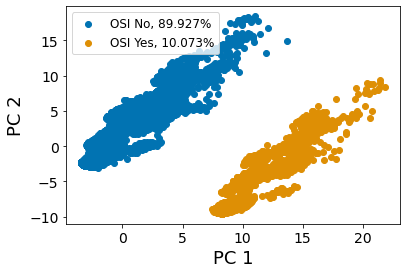
\includegraphics[width=\textwidth]{pca_osi.png}
		\subcaption{2-dimensional PCA projection colored by OSI}\label{fig:pca_osi}
	\end{minipage}
	\caption{2-dimensional PCA projection and two natural clusters}\label{fig:pca}
\end{figure}

\section{Modeling: Results and Discussion}\label{sec:model}

In this section, we fit models to predict whether patients have a ciTBI outcome from their covariates. We consider several models: $\ell_1$-penalized logistic regression \cite{simon2013sparse}, group $\ell_1$-penalized logistic regression \cite{simon2013sparse}, a single decision tree \cite{safavian1991survey}, a random forest \cite{ho1995random}, AdaBoost \cite{schapire2013explaining}, LogitBoost \cite{cai2006using}, and a linear SVM \cite{boser1992training}. All of these models were chosen for their relative ease of implementation and interpretability. As all of these algorithms have one or more parameters that can be tuned, based on practitioner feedback, we chose to operate at a point wherein the sensitivity was at least $0.95$ (or as close to it as possible) and the negative predictive value (NPV) was as close to $1$ as possible. We continue with the data split of age $< 2$ and $\geq 2$ and fit models for each group; we also fit models for the entire, unsplit dataset. The unsplit models can be thought of as a stability and reality check for whether the age-based demarcation is significant and necessary. 

\subsection{Baseline Model} \label{ssec:baseline}

Before proceeding, we briefly describe the model from \cite{kuppermann2009identification}, hereafter referred to as the baseline model. The model consists of two decision trees: one for patients with an age under $2$ years, and one for patients aged two years or older. The tree for patients younger than $2$ consists of questions about the presence of: an altered mental status (AMS), scalp hematoma, loss of consciousness for greater than $5$ seconds, a severe cause of injury, a palpable or possible skull fracture, and abnormal behavior per a parent. The questions are asked in the given order, and the presence of a `yes' answer to any leads to a possible ciTBI diagnosis and hence a CT scan; if all answers are `no', no scan is recommended. For patients older than $2$, the tree consists of questions about the presence of: an altered mental status (AMS), loss of consciousness, a history of vomiting, a severe cause of injury, a palpable or possible skull fracture, signs of a basilar skull fracture, and the presence of a severe headache. Once again, any `yes' answer leads to a scan, and all `no' answers leads to no scan. 

\subsection{Results} \label{ssec:results}

In Table \ref{tab:val_performance}, we present results for all of the algorithms on the validation set. That is, we trained all algorithms on the training set for a wide variety of parameters (if there were any), selected an appropriate operating point/threshold as described above on the validation set, and have summarized the selected operating points for each algorithm. We see that $\ell_1$-penalized Logistic Regression has the highest AUC while having a sensitivity close to the desired value of $0.95$ and an NPV close to $1$. Moreover, relative to other algorithms with similar characteristics (e.g., the Group $\ell_1$-penalized Logistic Regression and AdaBoost), we see that the specificity is much higher. Hence, we selected $\ell_1$-penalized Logistic Regression as our `best' method. Moreover, we see that this method performs much better than the baseline algorithm. In general, we see that the models trained on the unsplit (by age) data perform slightly worse than both of the models trained on the individual halves. 
\begin{table}[h]
\resizebox{\textwidth}{!}{%
\begin{tabular}{llllllll}
Algorithm      & Age   & AUC   & Accuracy & Sensitivity & Specificity & NPV   & Balanced Accuracy \\
\hline
$\ell_1$-penalized Logistic Regression            & young & 0.938 & 0.764    & 1.0         & 0.762       & 1.0   & 0.881             \\
$\ell_1$-penalized Logistic Regression             & old   & 0.931 & 0.751    & 0.957       & 0.75        & 1.0   & 0.854             \\
$\ell_1$-penalized Logistic Regression             & all   & 0.917 & 0.75     & 0.952       & 0.748       & 0.999 & 0.85              \\
Group $\ell_1$-penalized Logistic Regression & young & 0.908 & 0.728    & 1.0         & 0.726       & 1.0   & 0.863             \\
Group $\ell_1$-penalized Logistic Regression & old   & 0.917 & 0.68     & 0.957       & 0.678       & 1.0   & 0.818             \\
Group $\ell_1$-penalized Logistic Regression & all   & 0.917 & 0.745    & 0.952       & 0.743       & 0.999 & 0.848             \\
AdaBoost       & young & 0.781 & 0.064    & 1.0         & 0.058       & 1.0   & 0.529             \\
AdaBoost       & old   & 0.872 & 0.25     & 0.957       & 0.245       & 0.999 & 0.601             \\
AdaBoost       & all   & 0.899 & 0.59     & 0.952       & 0.587       & 0.999 & 0.77              \\
LogitBoost     & young & 0.825 & 0.889    & 0.714       & 0.891       & 0.998 & 0.802             \\
LogitBoost     & old   & 0.814 & 0.213    & 0.957       & 0.208       & 0.998 & 0.583             \\
LogitBoost     & all   & 0.746 & 0.198    & 0.952       & 0.191       & 0.998 & 0.572             \\
Decision Tree  & young & 0.898 & 0.118    & 0.929       & 0.113       & 0.996 & 0.521             \\
Decision Tree  & old   & 0.875 & 0.724    & 0.957       & 0.722       & 1.0   & 0.84              \\
Decision Tree  & all   & 0.809 & 0.01     & 0.988       & 0.0         & 0.75  & 0.494             \\
Random Forest  & young & 0.815 & 0.844    & 0.714       & 0.845       & 0.998 & 0.779             \\
Random Forest  & old   & 0.889 & 0.796    & 0.894       & 0.795       & 0.999 & 0.844             \\
Random Forest  & all   & 0.845 & 0.816    & 0.798       & 0.816       & 0.998 & 0.807             \\
Linear SVM            & young & 0.275 & 0.014    & 1.0         & 0.008       & 1.0   & 0.504             \\
Linear SVM            & old   & 0.645 & 0.057    & 0.957       & 0.051       & 0.994 & 0.504             \\
Linear SVM            & all   & 0.644 & 0.063    & 0.952       & 0.054       & 0.991 & 0.503             \\
Baseline       & young & 0.903 & 0.05     & 1.0         & 0.044       & 1.0   & 0.522             \\
Baseline       & old   & 0.869 & 0.615    & 0.957       & 0.613       & 0.999 & 0.785            
\end{tabular} }
\caption{Algorithm performance on validation data for each data split}\label{tab:val_performance}
\end{table}

We note that the group $\ell_1$-penalized Logistic Regression performed almost as well as the $\ell_1$-penalized Logistic Regression. However, this method is extremely sensitive to the regularization parameter, and we suspect that slight changes in the data used for training would lead to vastly different results. This result is unfortunate, as in principle, the grouping would allow us to enforce sparsity across a group of covariates (e.g., everything vomit related) and hence improve interpretability. We note that the decision tree also performed well (recall that the baseline model is also a decision tree), but that the logistic regression was better. Also, decision trees can heavily depend on the training data in ways that regression models do not. The random forest and boosted models (AdaBoost and LogitBoost) do not perform as well; we noticed that the performance was not linear in the number of trees, and conjecture that there may be some degree of overfitting on the training data. Either way, an ensemble model is naturally harder to interpret than a linear model. The SVM performed quite poorly, in contrast---it is generally surprising that a logistic regression method performs well where a linear SVM does not, but we chose not to investigate further given time and space constraints. 

Hence, we summarize results for $\ell_1$-regularized Logistic Regression and the baseline models on the test set in Table \ref{tab:test_performance}. We found that the regularization parameters for both the young and old models were $\approx 0.336$ and that the parameter for the model trained on the unsplit data was $\approx 1.129$. We see that the test sensitivity is close to $0.95$ and that the NPV is still close to $1$, and that the AUC is close to $0.85$; these numbers are a slight drop from the validation results, but are still good---in particular, they are much better than the baseline model. Once again, we see that the model trained on the unsplit (by age) data performs slightly worse than both of the models trained on the individual halves. Recalling Figure \ref{fig:pca}, wherein we saw a significant clustering effect based on OSI, we note that OSI and classification accuracy are not well correlated. 
\begin{table}[h]
\resizebox{\textwidth}{!}{%
\begin{tabular}{llllllll}
Algorithm & Age   & AUC   & Accuracy & Sensitivity & Specificity & NPV   & Balanced Accuracy \\
\hline
$\ell_1$-penalized Logistic Regression         & young & 0.846 & 0.772    & 0.923       & 0.77        & 0.999 & 0.846             \\
$\ell_1$-penalized Logistic Regression         & old   & 0.848 & 0.762    & 0.937       & 0.76        & 0.999 & 0.848             \\
$\ell_1$-penalized Logistic Regression         & all   & 0.822 & 0.794    & 0.85        & 0.793       & 0.999 & 0.822             \\
Baseline  & young & 0.875 & 0.054    & 1.0         & 0.042       & 1.0   & 0.521             \\
Baseline  & old   & 0.873 & 0.639    & 0.937       & 0.636       & 0.999 & 0.786            
\end{tabular}}
\caption{Algorithm performance on test data for each data split}\label{tab:test_performance}
\end{table}

\subsection{Discussion of the $\ell_1$-regularized Logistic Regression model} \label{ssec:discuss}

In this section, we provide some insights from studying the logistic regression models that we have fit. We note that this from of model is a good choice, as it is naturally interpretable: the $\ell_1$-penalization leads to naturally sparse coefficient vectors, so that only a subset of features are used in prediction. The sparsity combined with the linear nature of the classifier means that the coefficients' magnitudes have meaning, and the form of the model means that the odds ratio is a linear function of the data---this model is hence easy to use. 

In Figure \ref{fig:lr_ft_young}, \ref{fig:lr_ft_old}, and \ref{fig:lr_ft_all}, we provide computed feature importances from the model. That is, we report the magnitude of coefficients times the standard deviation (on the validation set) of the features. We see that across all of the data splits, AMS (altered mental state) is an important variable, as are various features related to vomit, hematoma location, and loss of consciousness. 
\begin{figure}
	\centering
	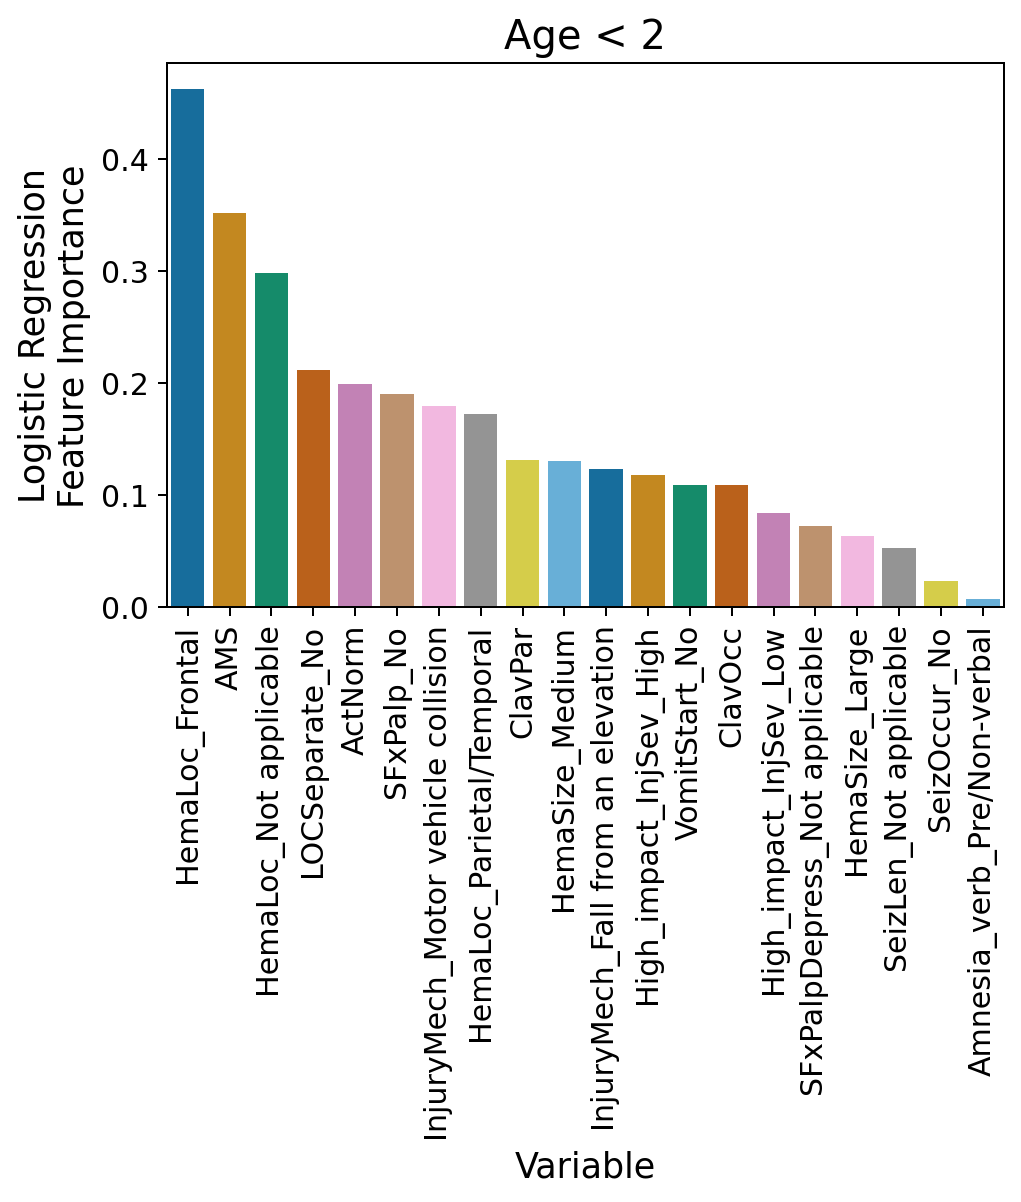
\includegraphics[width=0.7\textwidth]{lr_feat_importance_young.png}
	\caption{Feature importances from the $\ell_1$-regularized Logistic Regression for young patients}\label{fig:lr_ft_young}
\end{figure}
\begin{figure}
	\centering
	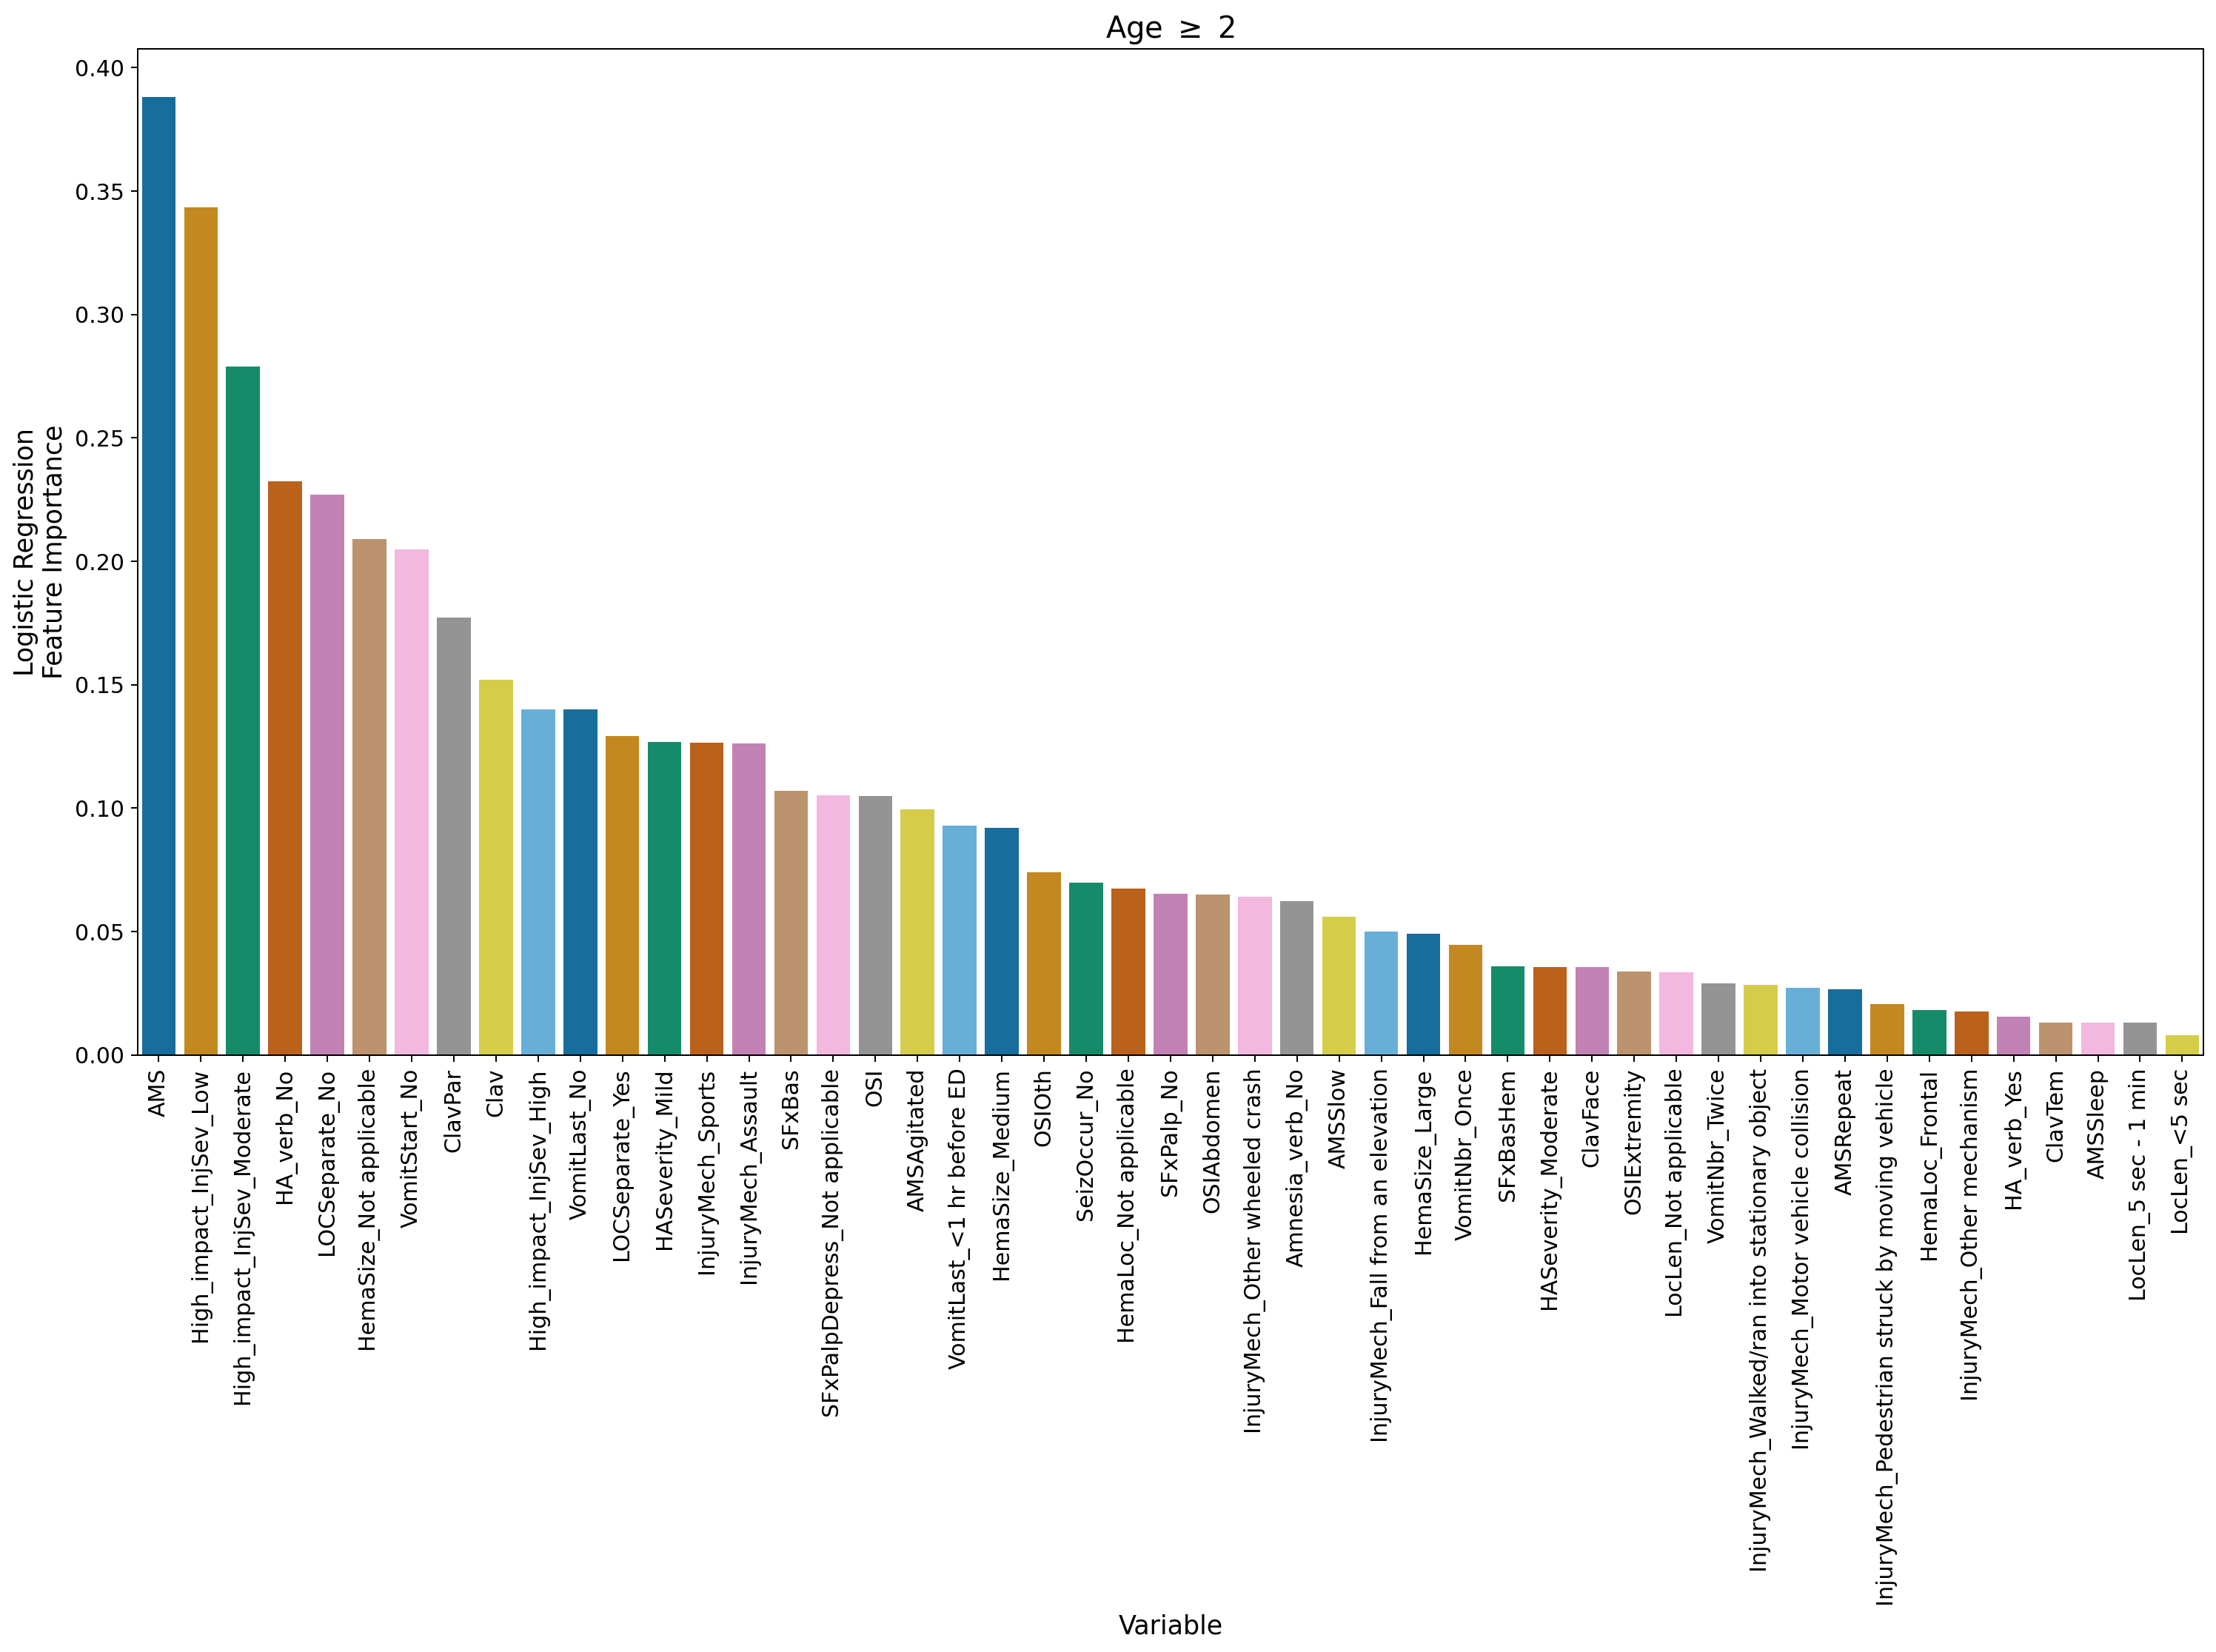
\includegraphics[width=\textwidth]{lr_feat_importance_old.png}
	\caption{Feature importances from the $\ell_1$-regularized Logistic Regression for older patients}\label{fig:lr_ft_old}
\end{figure}
\begin{figure}
	\centering
	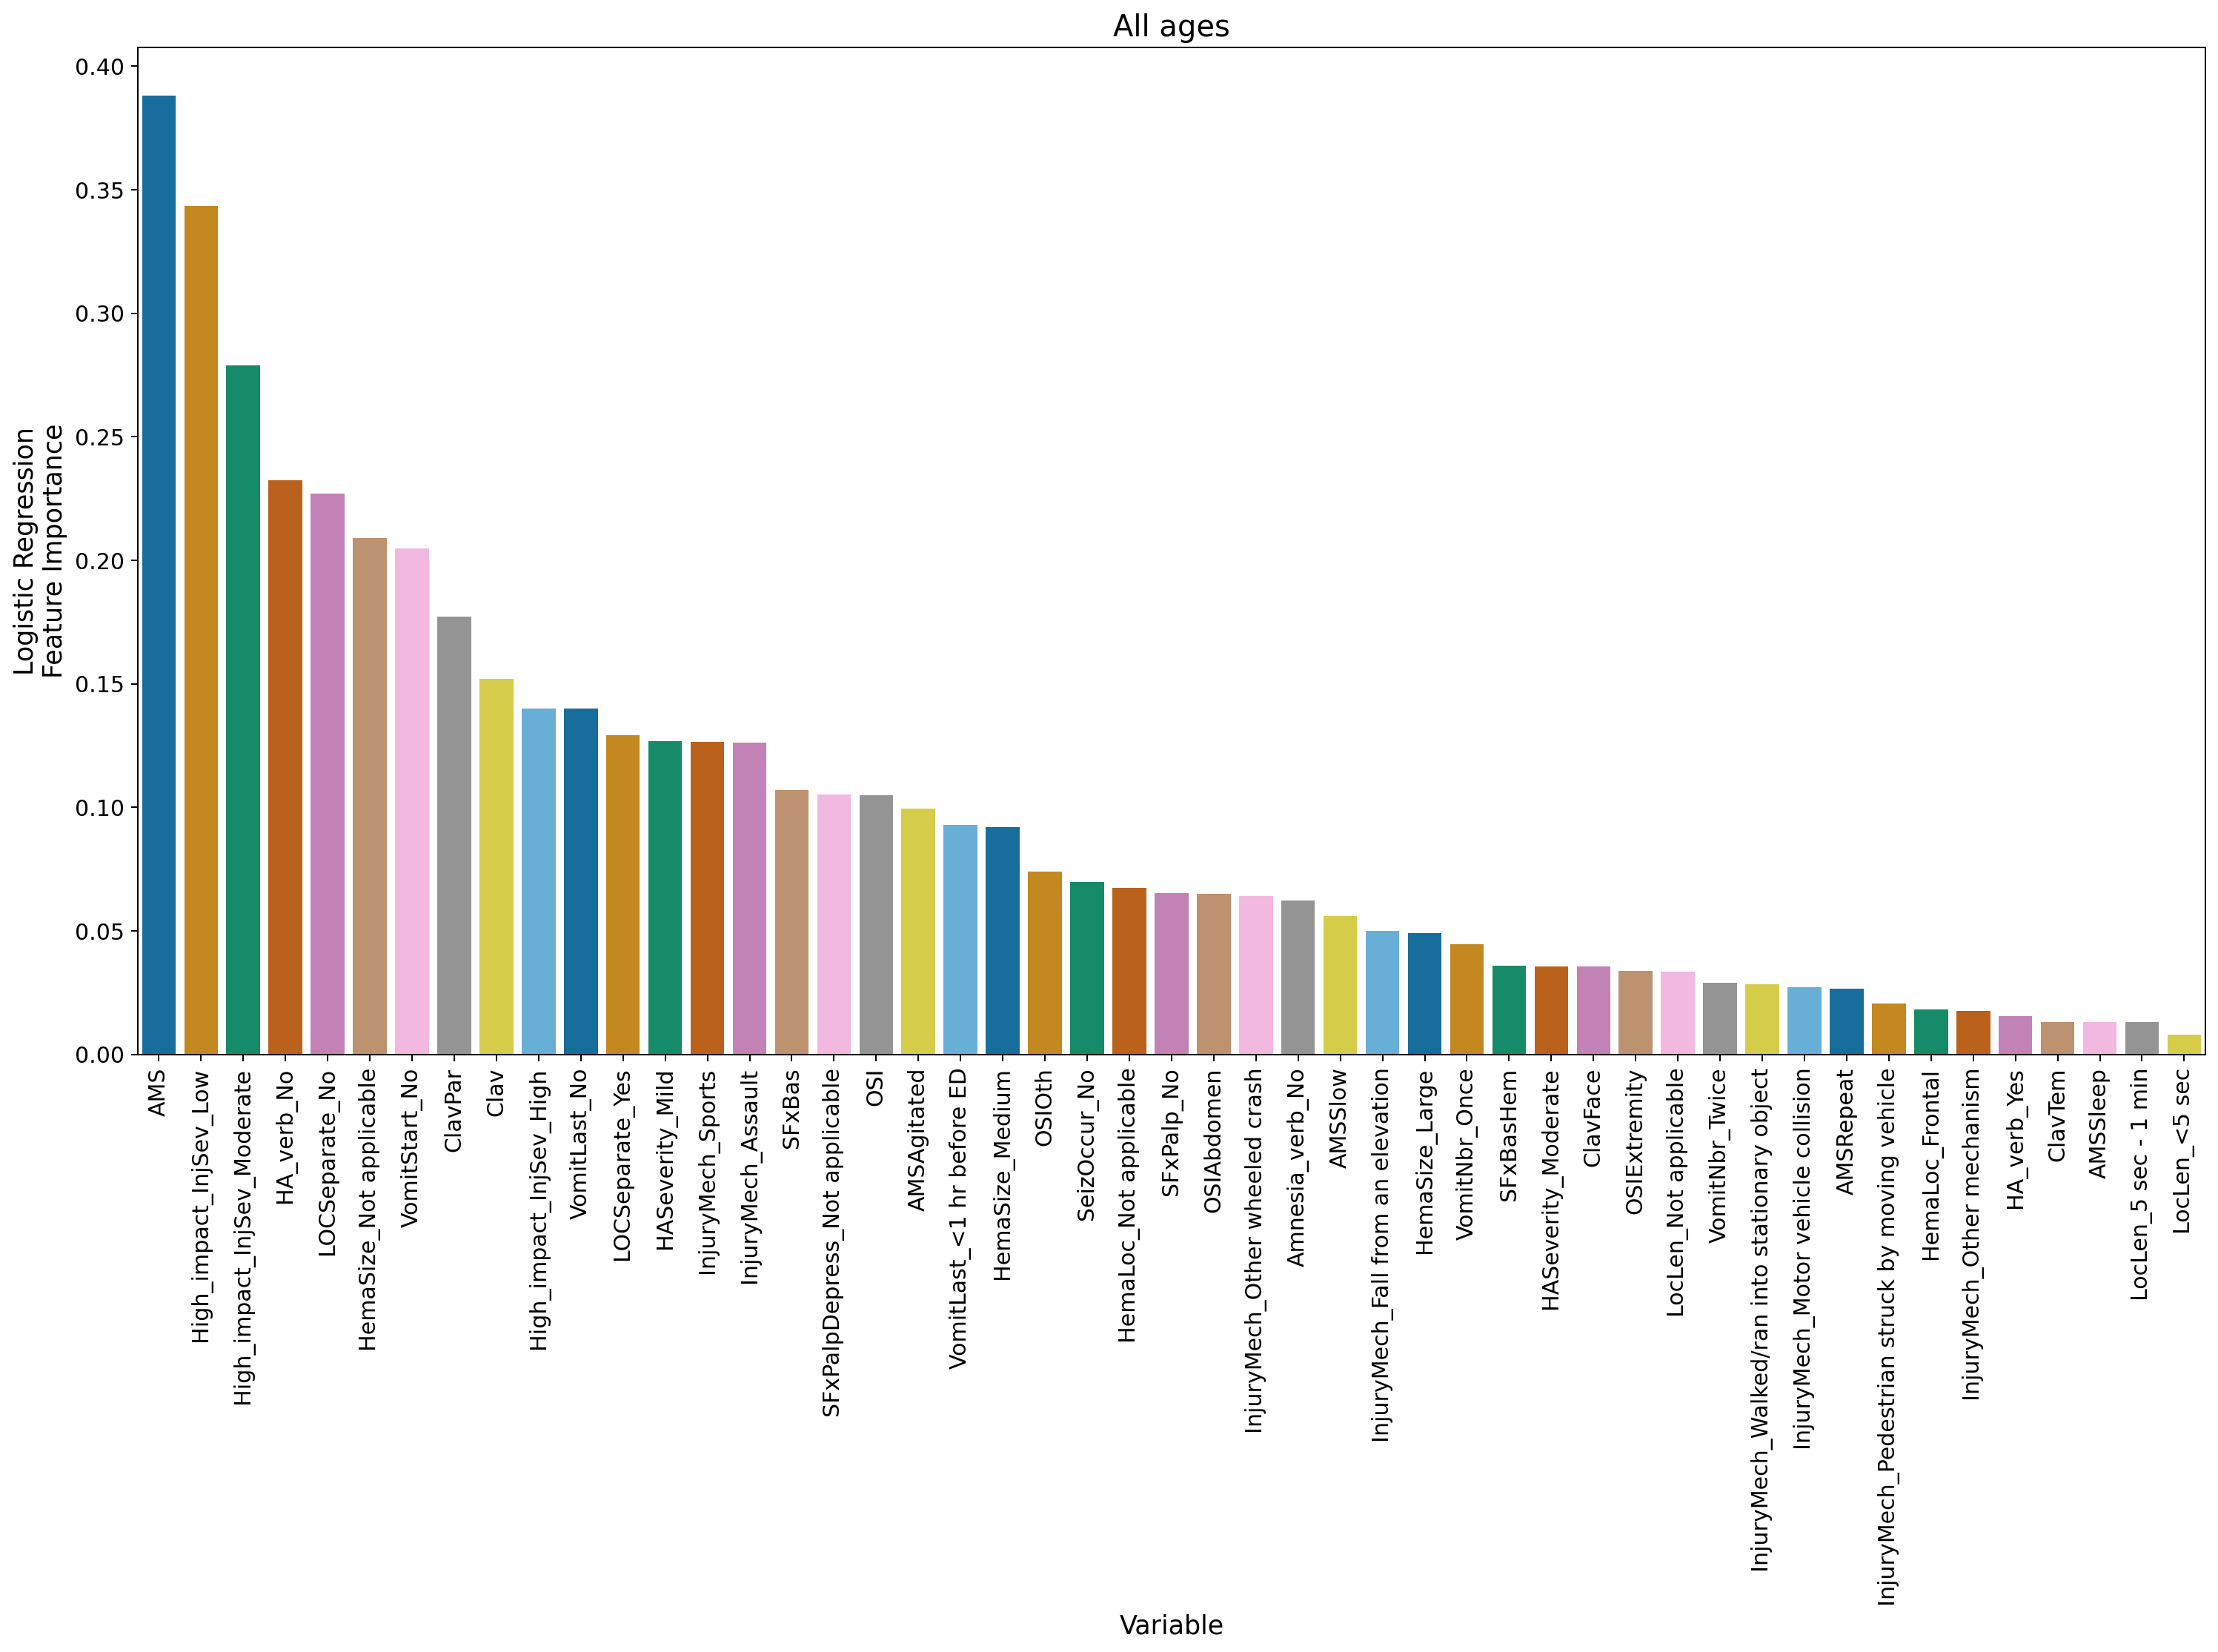
\includegraphics[width=\textwidth]{lr_feat_importance_all.png}
	\caption{Feature importances from the $\ell_1$-regularized Logistic Regression for all patients}\label{fig:lr_ft_all}
\end{figure}

In Figure \ref{fig:lr_roc}, we present ROC curves for the $\ell_1$-regularized Logistic Regression for the validation and the test data. We see that all of the logistic regression models are better than the baseline model, and that the ROC curves are far from the 45-degree line. 
\begin{figure}
	\begin{minipage}[b]{0.5\linewidth}
		\centering
		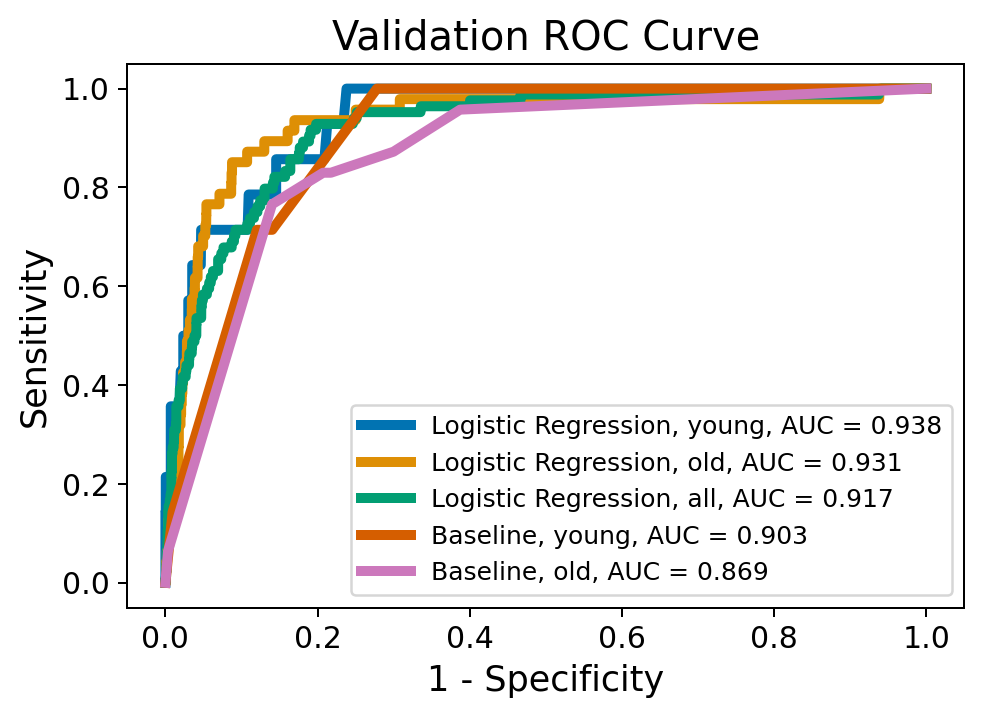
\includegraphics[width=\textwidth]{lr_val_roc.png}
		\subcaption{ROC curve on the validation data for the $\ell_1$-regularized Logistic Regression model}\label{fig:lr_val_roc}
	\end{minipage}%
	\begin{minipage}[b]{0.5\linewidth}
		\centering
		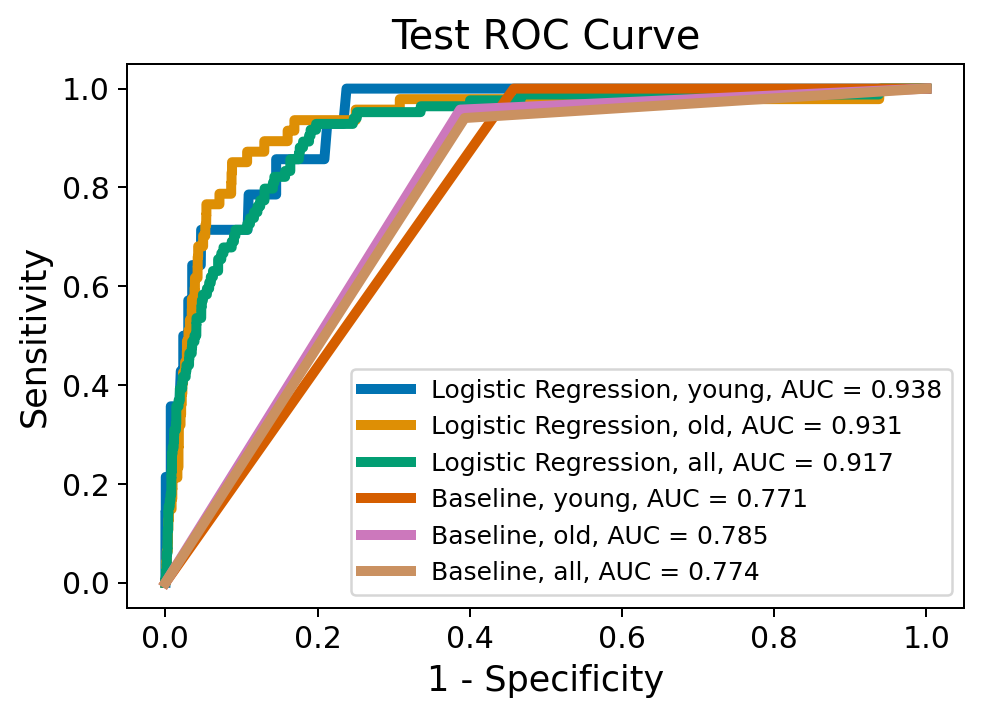
\includegraphics[width=\textwidth]{lr_test_roc.png}
		\subcaption{ROC curve on the test data for the $\ell_1$-regularized Logistic Regression model}\label{fig:lr_test_roc}
	\end{minipage}
	\caption{ROC curves for the $\ell_1$-regularized Logistic Regression model}\label{fig:lr_roc}
\end{figure}

Finally, in Figure \ref{fig:lr_lambda_auc}, we study the validation AUC as a function of the regularization strength. We see that in a neighborhood of the chosen value ($[10^{-1}, 10^{1/2}]$), the AUC is relatively stable and high. That is, perturbations to the regularization parameter or not searching on a fine enough grid are not concerns in our analysis. 
\begin{figure}
	\centering
	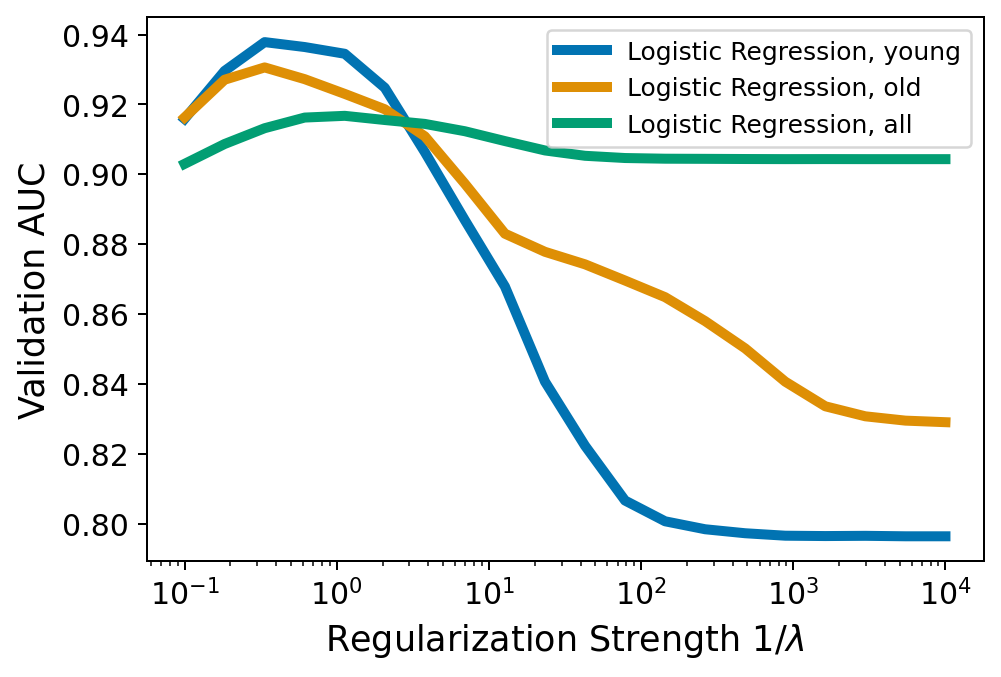
\includegraphics[width=0.7\textwidth]{lr_auc_lambda.png}
	\caption{Validation AUC for the $\ell_1$-regularized Logistic Regression as a function of regularization strength}\label{fig:lr_lambda_auc}
\end{figure}

\subsubsection{Model stability}

In this section, we report the results from bootstrapping the training dataset and evaluating the bootstrapped logistic regression models on the validation set. We measure the validation AUC as well as track which regularization parameter led to the best model. Ideally, we would see a tight concentration close to and around the previously observed values. As this step involves a parameter sweep, we used 20 bootstrap samples of size equal to a quarter of the original dataset and searched over 20 values of the regularization parameter. Our results appear in Figure \ref{fig:lr_bootstrap_val}, where we see that all of the AUCs have relatively tight concentration around the previously observed values. Moreover, the chosen regularization parameters are still close to the values picked for the chosen model. We present the mean and standard deviation of the bootstrapped validation AUCs in Table \ref{tab:bs_auc}: the values are consistent with what we saw earlier on the full dataset. 
\begin{table}[h]
\begin{tabular}{llll}
Age & Mean AUC & Standard Deviation of AUC & Model AUC (full data) \\
\hline
Young & 0.909 & 0.0172 & 0.938 \\
Old & 0.905 & 0.0124 & 0.931 \\
All & 0.892 & 0.009933 & 0.917 
\end{tabular}
\caption{Bootstrapped mean and standard deviation of validation AUCs for the $\ell_1$-regularized Logistic Regression model; note that the 20 bootstrapped datasets were of smaller size (one quarter) than the original data.}\label{tab:bs_auc}
\end{table}

\begin{figure}
	\centering
	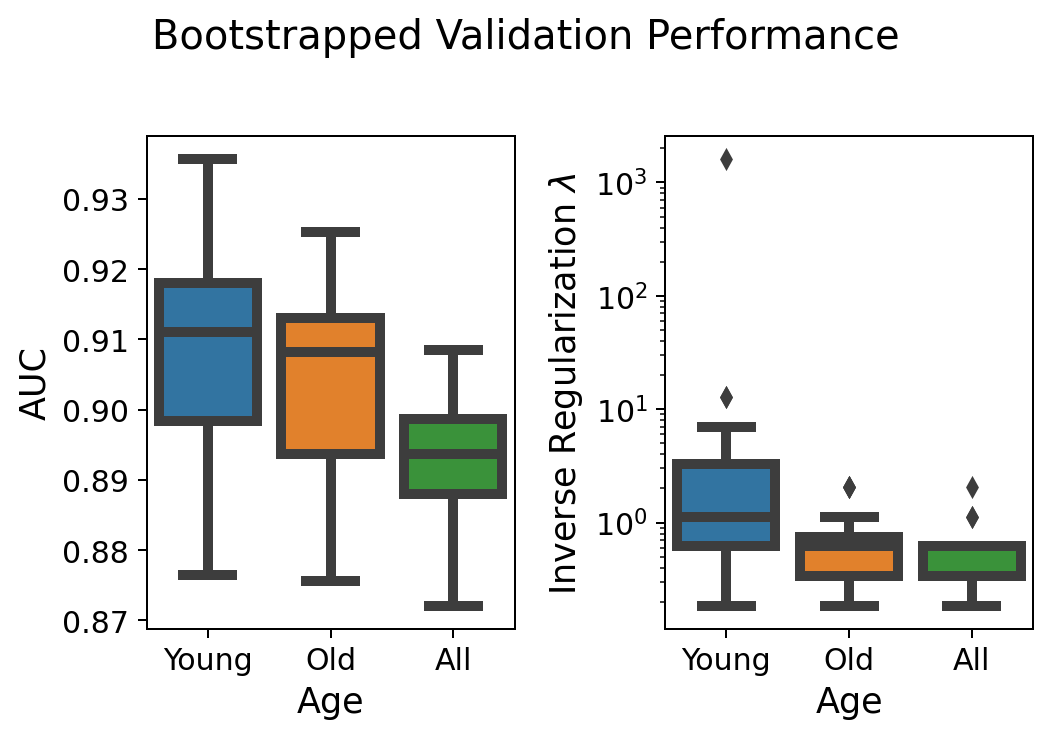
\includegraphics[width=0.7\textwidth]{lr_bootstrap_val.png}
	\caption{Bootstrapped validation AUC for the $\ell_1$-regularized Logistic Regression and the corresponding regularization parameters. Recall that the young and old models previously had parameters of $0.336$ and the all model had a parameter value of $1.129$.}\label{fig:lr_bootstrap_val}
\end{figure}

\subsection{A different data split: Pre-verbal v. verbal} \label{ssec:verbal}

In this section, we return to Figure \ref{fig:preverbal}, where we saw that many patients under the age of $5$ were pre-verbal, but the standard practice is to separate subjects before and after the age of $2$. Moreover, there were relatively few patients over the age of $5$ that were not verbal (104 subjects in validation), so we conjecture that a rule split based on pre-verbal v. verbal status might be a better choice. Using the same train/validation/test splits, we re-trained our $\ell_1$-regularized Logistic Regression models. 

In Figure \ref{fig:lr_roc_vb}, we present ROC curves for the $\ell_1$-regularized Logistic Regression for the validation and the test data with the new data split. We see that all of the logistic regression models are better than the baseline model, and that the ROC curves are far from the 45-degree line, but that this split leads to slightly worse performance than the original division at the age of $2$. Nonetheless, we believe that this or similar data splits merit further investigation: there are children under the age of two that are verbal and can hence communicate their mental status, but there are also those over the age of two that are not and hence cannot communicate. 
\begin{figure}
	\begin{minipage}[b]{0.5\linewidth}
		\centering
		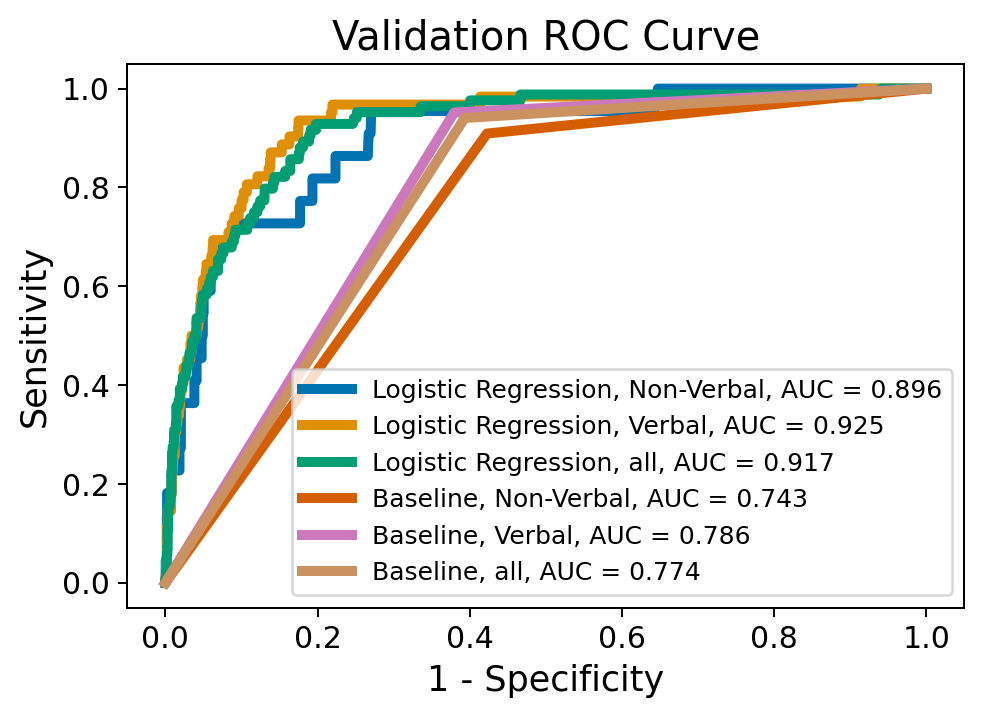
\includegraphics[width=\textwidth]{lr_val_roc_verbal.png}
		\subcaption{ROC curve on the validation data for the $\ell_1$-regularized Logistic Regression model}\label{fig:lr_val_roc_vb}
	\end{minipage}%
	\begin{minipage}[b]{0.5\linewidth}
		\centering
		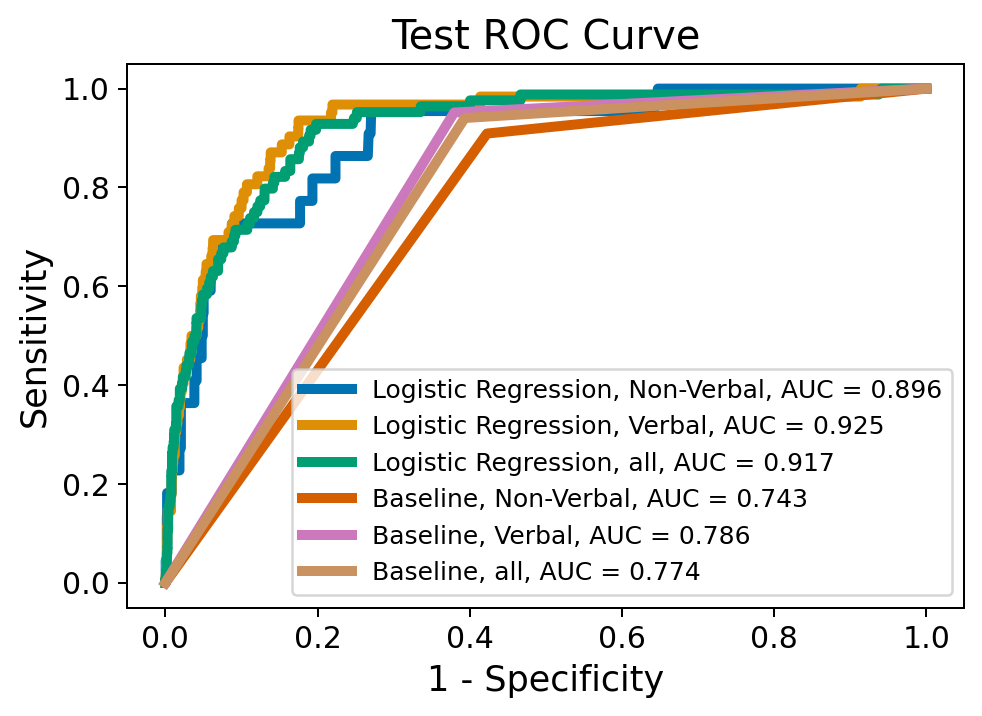
\includegraphics[width=\textwidth]{lr_test_roc_verbal.png}
		\subcaption{ROC curve on the test data for the $\ell_1$-regularized Logistic Regression model}\label{fig:lr_test_roc_vb}
	\end{minipage}
	\caption{ROC curves for the $\ell_1$-regularized Logistic Regression model with the pre-verbal/verbal split}\label{fig:lr_roc_vb}
\end{figure}

\section{Conclusions} \label{sec:conclusions}

In this report, we have looked at patient data from a prospective cohort study wherein patients between the ages of 0-17 who visited one of a series of hospitals presenting with a potential TBI were enrolled. We were given data from patient questionnaires that was converted to numerical features and fit models to predict the need for a CT scan. We found that an $\ell_1$-penalized logistic regression model performed the best and outperformed the model derived in  \cite{kuppermann2009identification}. 

There are many threads left unfinished in this work, mostly because of time and space constraints. First, it would be interesting to systematically investigate whether a better age cutoff (in terms of model performance) could be obtained, or whether an age cutoff combined with some other factor (like pre-verbal v. verbal) would be better. Additionally, it would be good to compare additional models and to investigate the performance and utility of some model explainability techniques, like LIME \cite{ribeiro2016should} or SHAP \cite{vstrumbelj2014explaining}. 


\subsection{Division of Labor}

Hyunsuk Kim contributed to the exploratory data analysis, implemented the $\ell_1$-penalized logistic regression, grouped $\ell_1$-penalized logistic regression, consolidated everyone's model code into one larger wrapper function, worked on the baseline model, edited and coded functions to find the statistical metrics saved by each of the models, and offered comments on the final report.

Mark Oussoren contributed to much of the exploratory data analysis, did much of the data processing and implementation of dataset.py, worked on coding the baseline model, summarized his findings for EDA and the baseline model, and documented the judgement calls made working with this data set, and offered comments on the final report.

Sahil Saxena created a slide deck to share with our clinician contact, implemented an SVM model and looked at the effect of different kernels and how SVM works on the first few PCA components, contributed to the data dictionary and README files, and offered comments on the final report.

Florica Constantine acted as the project lead overseeing the project, editing others results across all aspects of the project, and also individually worked on much of the exploratory data analysis, implemented the boosting models, implemented the stability analysis, wrote the final report, implemented \texttt{model\_best.py} and \texttt{baseline.py}, and offered comments on the final report.

\printbibliography

\end{document}  
